% MedVision Draft V1 is a journal-neutral two-column manuscript.
% The verified MedVision_JBI_V2 source and outputs remain unchanged.

\documentclass[10pt,a4paper,twocolumn]{article}

\usepackage[margin=2.35cm,columnsep=0.72cm]{geometry}
\usepackage{amsmath,amssymb}
\usepackage{booktabs}
\usepackage{array}
\usepackage{float}
\usepackage{placeins}
\usepackage{graphicx}
\usepackage{multirow}
\usepackage[numbers,sort&compress]{natbib}
\usepackage{xcolor}
\usepackage{microtype}
\usepackage{caption}
\usepackage{url}
\usepackage{hyperref}
\usepackage{balance}
\hypersetup{hypertexnames=false,hidelinks}
\Urlmuskip=0mu plus 2mu\relax

\graphicspath{{figures/}}
\setlength{\floatsep}{7pt plus 2pt minus 2pt}
\setlength{\textfloatsep}{8pt plus 2pt minus 2pt}
\setlength{\intextsep}{7pt plus 2pt minus 2pt}
\setcounter{topnumber}{5}
\setcounter{dbltopnumber}{5}
\renewcommand{\topfraction}{0.95}
\renewcommand{\dbltopfraction}{0.95}
\renewcommand{\textfraction}{0.05}
\renewcommand{\floatpagefraction}{0.80}
\renewcommand{\dblfloatpagefraction}{0.80}
\setlength{\columnsep}{0.72cm}
\setlength{\parindent}{1em}
\setlength{\parskip}{0pt}
\linespread{1.10}
\interfootnotelinepenalty=10000
\captionsetup{font=small,labelfont=bf,labelsep=period}
\renewcommand{\figurename}{Fig.}

\title{Auditing Image Use in Medical Vision Language Models}
\author{Nafis Al Rahman \and Tanvir Mahmud}
\date{}

\begin{document}
\raggedbottom

\twocolumn[{
\begin{@twocolumnfalse}
\maketitle
\vspace{-1.5em}
\begin{abstract}
Medical vision-language models can obtain strong classification scores from
radiology reports even when their corresponding images contribute little to
the decision. This risk is greatest when evaluation labels and text inputs
share report provenance. We audited five fusion conditions on 2,953 frontal
MIMIC-CXR studies divided at patient level into 2,049 training, 449 validation,
and 455 test studies. The primary intervention replaced each radiograph with a
constant gray image while preserving its report, target, architecture, and
evaluation cohort. The Image Contribution Metric (ICM) measured the relative
Macro-F1 change between the full model and this report-preserving control.
Across eight baseline seeds, Macro-F1 was $0.9397\pm0.0061$, whereas the
retained Gray-Square control achieved 0.9381. Baseline ICM was
$0.0016\pm0.0065$ with a 95\% bootstrap confidence interval of
$[-0.0026,0.0061]$. A signed-rank test did not reject zero ($p=0.4219$), and
two one-sided tests supported equivalence inside the operational interval
$[-0.01,0.01]$ ($p=0.0040$). None of the tested interventions produced a
robust increase in incremental image contribution. The product-of-experts
condition increased expected calibration error from 0.0237 to 0.0621, while
retained baseline gates stayed close to their initial values, with an overall
mean of 0.49975. These findings show that high multimodal performance can
coexist with negligible change after image replacement. ICM, matched
interventions, calibration, and gate inspection provide complementary checks
for this form of benchmark dependence. The conclusion is limited to the
report-linked cohort and retained implementation and does not imply that chest
radiographs lack diagnostic value.
\end{abstract}

\noindent\textbf{Keywords:} medical vision-language model; label circularity;
shortcut learning; modality audit; Image Contribution Metric; equivalence
testing; MIMIC-CXR.
\vspace{1.2em}
\end{@twocolumnfalse}
}]

\section{Introduction}\label{sec:introduction}

Chest radiography is interpreted in a clinical information environment rather
than as an isolated image. Radiologists draw on image appearance, indication,
prior examinations, and other contextual information before expressing their
assessment in a report. Medical vision-language models (VLMs) mirror part of
that workflow by combining a radiograph with its report or another clinical
text source. Large paired resources such as MIMIC-CXR make this combination
possible at scale and have supported classification, representation learning,
report generation, and question answering \cite{johnson2019mimiccxr}. The
appeal is clear: an image can carry anatomical and pathological evidence while
text can represent symptoms, uncertainty, and prior interpretation.

The success of paired pretraining has strengthened this view. ConVIRT learns
visual representations from image-text agreement, GLoRIA models global and
local correspondence, and BioViL emphasizes biomedical report semantics
\cite{zhang2022convirt,huang2021gloria,boecking2022textsemantics}. Clinical
language encoders further improve the representation of medical terminology,
negation, and contextual phrases \cite{devlin2019bert,alsentzer2019clinicalbert}.
These developments establish that reports are useful supervision and useful
inputs. They do not establish that both modalities affect a particular
downstream prediction. A model can be multimodal by construction while behaving
like a unimodal model on the evaluated endpoint.

This distinction matters because predictive performance is a property of a
model, a cohort, and a target definition. It is not direct evidence about the
reason for a prediction. Deep networks often exploit shortcuts that remain
stable within a benchmark but fail to represent the intended clinical
construct \cite{geirhos2020shortcut}. In radiology, scanner characteristics,
institutional practice, population composition, acquisition protocol, and
annotation procedure can all become predictive signals
\cite{gichoya2023shortcuts}. In a VLM, the report can form an additional shortcut
when it encodes most of the information rewarded by the label. The image branch
may then add little measurable information even though the architecture
contains a large visual encoder, cross-attention, and an explicit fusion gate.

Recent evidence shows why this possibility cannot be dismissed as an edge
case. Multimodal medical systems can return correct answers with flawed visual
rationales, and several chest-radiography models retain substantial performance
when visual information is removed or replaced
\cite{jin2024hiddenflaws,lotfinia2026needimage}. Clinical context can materially
change measured performance, so a headline score may partly describe the
informativeness of the supplied context rather than visual recognition
\cite{wang2026clinicalcontext}. Audit frameworks have consequently begun to
separate answer accuracy from modality dependence and to identify settings in
which apparently successful models occupy a dangerous combination of high
performance and weak visual grounding
\cite{sadanandan2026consistentdangerous}. The common implication is that image
use should be measured through intervention rather than inferred from model
components or explanations.

Target provenance creates a particularly direct threat in MIMIC-CXR-derived
classification. CheXpert converts report language into uncertainty-aware
pathology labels \cite{irvin2019chexpert}. When the predictor also receives the
same report, or its \texttt{findings} section, the target and the text input
share a source. The resulting task may remain useful for studying report-linked
prediction, fusion behaviour, or computational auditing. It no longer isolates
independent recognition from the radiograph. A model can be rewarded for
recovering the linguistic evidence that contributed to label generation. Errors
or subgroup effects in natural-language labelers can also propagate into the
training target and the apparent model performance
\cite{sabottke2024targetselection,santomartino2024nlplabeling}.

This form of construct overlap complicates the interpretation of debiasing.
Methods developed for visual question answering often expose, down-weight, or
combine an easy language-only expert with a multimodal expert
\cite{agrawal2018dontassume,clark2019easyway,cadene2019rubi}. Those methods are
well motivated when the language pathway captures a nuisance prior. In a
report-derived classification task, however, the language pathway can be close
to the mechanism that produced the reference label. Penalizing it may lower the
score or distort confidence without generating additional visual information.
The result cannot be interpreted as better image use unless an image-preserving
comparison demonstrates that change. Prototype and counterfactual methods can
improve transparency, but explanation quality and causal input dependence
remain separate questions \cite{chiang2026cxrnexus}.

Three gaps motivate the present study. First, modality controls are often not
matched closely enough to the full model. Removing the report, training a new
unimodal architecture, or using a different cohort changes more than the
availability of image information. A report-preserving image intervention
provides a cleaner contrast because the report, target, evaluation cases, and
multimodal path remain fixed. Second, fusion parameters and saliency maps are
frequently read as evidence of reliance. A balanced gate can remain close to its
initial value, and an attention or activation map can look plausible even when
the prediction barely changes after image replacement
\cite{arevalo2017gmu,selvaraju2017gradcam}. Third, a non-significant difference
does not demonstrate negligible effect. Equivalence testing is needed when the
scientific question concerns whether an effect lies inside a prespecified
operational margin \cite{lakens2017equivalence}.

We therefore conduct a controlled modality audit on a three-class
MIMIC-CXR-derived task comprising Normal, Pneumonia, and Pneumothorax. The
baseline combines a DenseNet-121 image encoder and Bio\_ClinicalBERT report
encoder through cross-attention and a bounded per-class gate. Four additional
conditions test a learned text-prior product-of-experts design, a
noise-sensitivity (anti-consistency) objective, an exploratory grounding-aware
condition, and adaptive gating. The primary intervention replaces every
radiograph with a constant gray image while preserving the report. We define
the Image Contribution Metric (ICM) as the relative Macro-F1 difference between
the full model and this Gray-Square reference, then pair it with seed-level
uncertainty and two one-sided equivalence tests.

The analysis is organized around three questions. Does a real radiograph change
performance when the report remains available? Do the tested fusion and
debiasing conditions increase that incremental contribution? Do retained gate
values and qualitative saliency provide evidence consistent with the
behavioural intervention? Answering these questions requires performance,
calibration, paired testing, per-class error analysis, and provenance to be read
together. The contribution is therefore an audit procedure and an empirical
case study of a report-linked benchmark. It is not a new diagnostic model, and
it does not imply that radiographs are unnecessary in clinical care.

\section{Related work}\label{sec:related-work}

This section places the audit between three research areas: medical image-text
representation learning, shortcut mitigation, and intervention-based model
evaluation. Table~\ref{tab:related-comparison} summarizes the closest methods
and identifies the evidence each contributes. The comparison is conceptual;
reported models use different datasets, targets, and evaluation designs and
their numerical results are not directly comparable.

\subsection{Medical image-text learning}

Large image-report collections allow supervision to be obtained from text that
already exists in clinical practice. ConVIRT uses paired contrastive learning
to align images and reports, GLoRIA combines global and local representations,
and BioViL strengthens the use of biomedical language semantics
\cite{zhang2022convirt,huang2021gloria,boecking2022textsemantics}. These methods
show that text can improve visual representations, especially when manual image
labels are scarce. They also illustrate why the evaluation target must be kept
distinct from the supervision source. A representation can encode useful image
content while a downstream classifier still relies mainly on report-derived
features.

Report encoders add another source of asymmetry. BERT and clinical-domain
variants encode lexical and contextual cues at a level that a relatively small
image branch may not match \cite{devlin2019bert,alsentzer2019clinicalbert}. In
radiology reports, explicit mentions, negation, and uncertainty can be closely
aligned with the output classes. If those same phrases were used to produce the
labels, a high score is expected from the language pathway. It is therefore
necessary to distinguish the benefit of text for prediction from evidence that
the image changed the prediction.

\subsection{Shortcut learning and language priors}

Shortcut learning provides the broader framework for this distinction.
Predictive systems may use features that work in a development distribution but
do not represent the intended task \cite{geirhos2020shortcut}. Radiology models
are exposed to many such features, including acquisition artifacts and
institution-specific correlations \cite{gichoya2023shortcuts}. A multimodal
model adds a more direct shortcut when one modality contains a near-explicit
description of the target.

Language-prior research in visual question answering offers several mitigation
strategies. VQA-CP changes train-test answer priors, ensemble approaches model
the easy route, and RUBi or product-of-experts losses reduce the influence of a
language-only component \cite{agrawal2018dontassume,clark2019easyway,
cadene2019rubi}. These designs assume that the language signal is predictive but
misleading. That assumption is weaker in report-linked radiology
classification. Here the report can be both clinically meaningful and
structurally connected to the label. Suppression may remove rewarded
information, but it cannot create an independent image reference standard.

\subsection{Circularity and modality audits}

Studies of medical VLMs increasingly test whether output quality reflects
visual evidence. Jin et al. separate correct answers from the quality of their
multimodal rationale, while Wang et al. show that the usefulness of context can
alter chest-radiography performance
\cite{jin2024hiddenflaws,wang2026clinicalcontext}. Lotfinia et al. use image
removal and related interventions across multiple systems, demonstrating that
text-only or visually disrupted conditions can remain competitive
\cite{lotfinia2026needimage}. Sadanandan and Behzadan organize such behaviour
into an audit taxonomy and motivate grounding-aware objectives
\cite{sadanandan2026consistentdangerous}. CXR-NeXus represents a complementary
direction based on prototypes and counterfactual consistency
\cite{chiang2026cxrnexus}.

These contributions shift attention from architecture labels to observable
behaviour. They also leave several design choices open. A control can be trained
separately or applied to a retained model; it can remove, replace, or permute an
input; and it can preserve or change the text pathway. Each choice answers a
different question. Our Gray-Square condition is deliberately narrow: it asks
how much Macro-F1 changes when image content is removed while the report-linked
input and the multimodal processing path remain available.

\subsection{Fusion parameters and explanations}

Gated multimodal units offer an interpretable-looking mechanism for balancing
modalities \cite{arevalo2017gmu}. The numerical gate is still a learned
parameter rather than a causal contribution estimate. It can remain near
initialization when signals are redundant, gradients are weak, or the loss is
already minimized through another route. Attention and Grad-CAM face a related
interpretive boundary. They can identify where a model produced high internal
activation, but a plausible map does not show how the output would change if
that evidence were absent \cite{selvaraju2017gradcam}. Reasoning-oriented and
prototype-based systems may make intermediate representations easier to
inspect, yet their explanations remain complementary to controlled ablation
\cite{myronenko2025reasoningcxr,chiang2026cxrnexus}.

\subsection{Statistical evidence for a negligible effect}

Modality audits often report a small difference followed by a conventional
test against zero. A non-significant result is ambiguous because it can reflect
either a small effect or insufficient precision. Equivalence testing reverses
the question by asking whether the effect and its uncertainty fit inside a
prespecified interval \cite{lakens2017equivalence}. This approach is useful for
ICM because the scientific claim concerns an operationally negligible change,
not exact mathematical equality. The margin must nevertheless be treated as a
study definition rather than a universal clinical threshold.

\begin{table*}[t]
\centering
\caption{Related methods and the evidence they provide.}
\label{tab:related-comparison}
\small
\setlength{\tabcolsep}{4pt}
\begin{tabular}{p{0.17\textwidth}p{0.19\textwidth}p{0.23\textwidth}p{0.32\textwidth}}
\toprule
Work & Primary setting & Relevant method & Relation to this audit \\
\midrule
ConVIRT \cite{zhang2022convirt} & Paired medical images and text & Contrastive representation learning & Establishes the value of report supervision but does not isolate image contribution in a report-linked classifier. \\
GLoRIA \cite{huang2021gloria} & Label-efficient image recognition & Global-local image-text alignment & Motivates cross-modal representation learning; alignment scores are not behavioural evidence of modality dependence. \\
BioViL \cite{boecking2022textsemantics} & Biomedical vision-language processing & Domain-specific text semantics & Supports the report encoder choice and illustrates the strength of the linguistic pathway. \\
VQA debiasing \cite{agrawal2018dontassume,clark2019easyway,cadene2019rubi} & Language priors in visual question answering & Prior balancing and product-of-experts training & Provides the LMH rationale, but its nuisance-prior assumption may not hold when reports generate labels. \\
Context audit \cite{wang2026clinicalcontext} & Chest-radiography models with clinical context & Comparison across context conditions & Shows that context changes measured performance and motivates explicit provenance analysis. \\
Image-removal audit \cite{lotfinia2026needimage} & Medical VLMs at multiple scales & Occlusion, replacement, and modality controls & Closest behavioural precedent; the present work adds relative ICM, equivalence testing, calibration, and gate extraction. \\
Grounding audit \cite{sadanandan2026consistentdangerous} & Multimodal medical AI & Audit taxonomy and grounding-aware objective & Motivates exploratory GACR-B and the separation of high performance from safe modality behaviour. \\
CXR-NeXus \cite{chiang2026cxrnexus} & Interpretable chest X-ray classification & Prototype memory and counterfactual consistency & Provides explanation-oriented evidence; the present intervention focuses on output sensitivity to image replacement. \\
\bottomrule
\end{tabular}
\end{table*}

The comparison also reveals a difference between representation-learning and
audit objectives. Representation-learning papers usually ask whether paired
text improves transfer, label efficiency, or downstream accuracy. An audit asks
whether the resulting predictor depends on the modality named in its claim.
Both questions are legitimate, but the first cannot answer the second without
an intervention. This is why a model that benefits from image-text pretraining
can still show little incremental image contribution on a later report-linked
classification task.

The same distinction applies to explanations. A rationale, prototype, or
activation map describes an internal or generated representation. A
counterfactual input comparison measures output sensitivity. Agreement between
the two strengthens an interpretation, while disagreement should be reported
rather than reconciled by assuming that the explanation is causal. The current
study gives priority to the Gray-Square comparison and treats Grad-CAM as a
limited qualitative check. This ordering follows the information available in
the retained outputs and avoids using saliency to compensate for a missing
behavioural effect.

Finally, prior work differs in the source of uncertainty it reports. Large
cross-model audits provide breadth across architectures, whereas repeated seeds
provide variation within an implementation. Subject-level paired tests assess
whether the same cases change, while equivalence tests address whether the
seed-level contribution lies inside an operational interval. The present design
does not replace broad external evaluation; it adds depth around a single
audited pipeline. Its main value is the explicit connection between target
provenance, image replacement, model-level replication, and statistical claim.

Taken together, prior work establishes the plausibility of text dominance and
the need for controlled interventions. The present study joins four evidence
types that are usually reported separately: a report-preserving image
intervention, a relative per-seed contribution measure, equivalence testing,
and inspection of retained fusion gates. The combined design is intended to
make the claim boundary visible: it evaluates image contribution to one
report-linked endpoint rather than visual competence in general.

\section{Methods}\label{sec:methods}

The methods follow the sequence in Fig.~\ref{fig:design}: define the
report-linked cohort, encode both modalities, compare controlled fusion
conditions, and evaluate every retained seed on the same test set. The primary
estimand is the incremental contribution of image content when report
information remains available. Discrimination, calibration, paired errors, and
gate behaviour provide supporting evidence but do not replace the
intervention-based comparison.

\subsection{Study design, data source, and cohort}\label{sec:study-design}

We performed a retrospective computational audit. The estimand was incremental
image contribution when the report remained available. The principal
intervention replaced each radiograph by a constant gray tensor while retaining
the report, target, fusion path, and evaluation cohort. Full multimodal outputs
were compared with this report-preserving control and with descriptive
text-only and image-only controls. Figure~\ref{fig:design} presents the image
pathway, report pathway, fusion design, and seed-level audit. The visual is a
conceptual overview; the retained implementation is specified below.

\begin{figure*}[t]
\centering
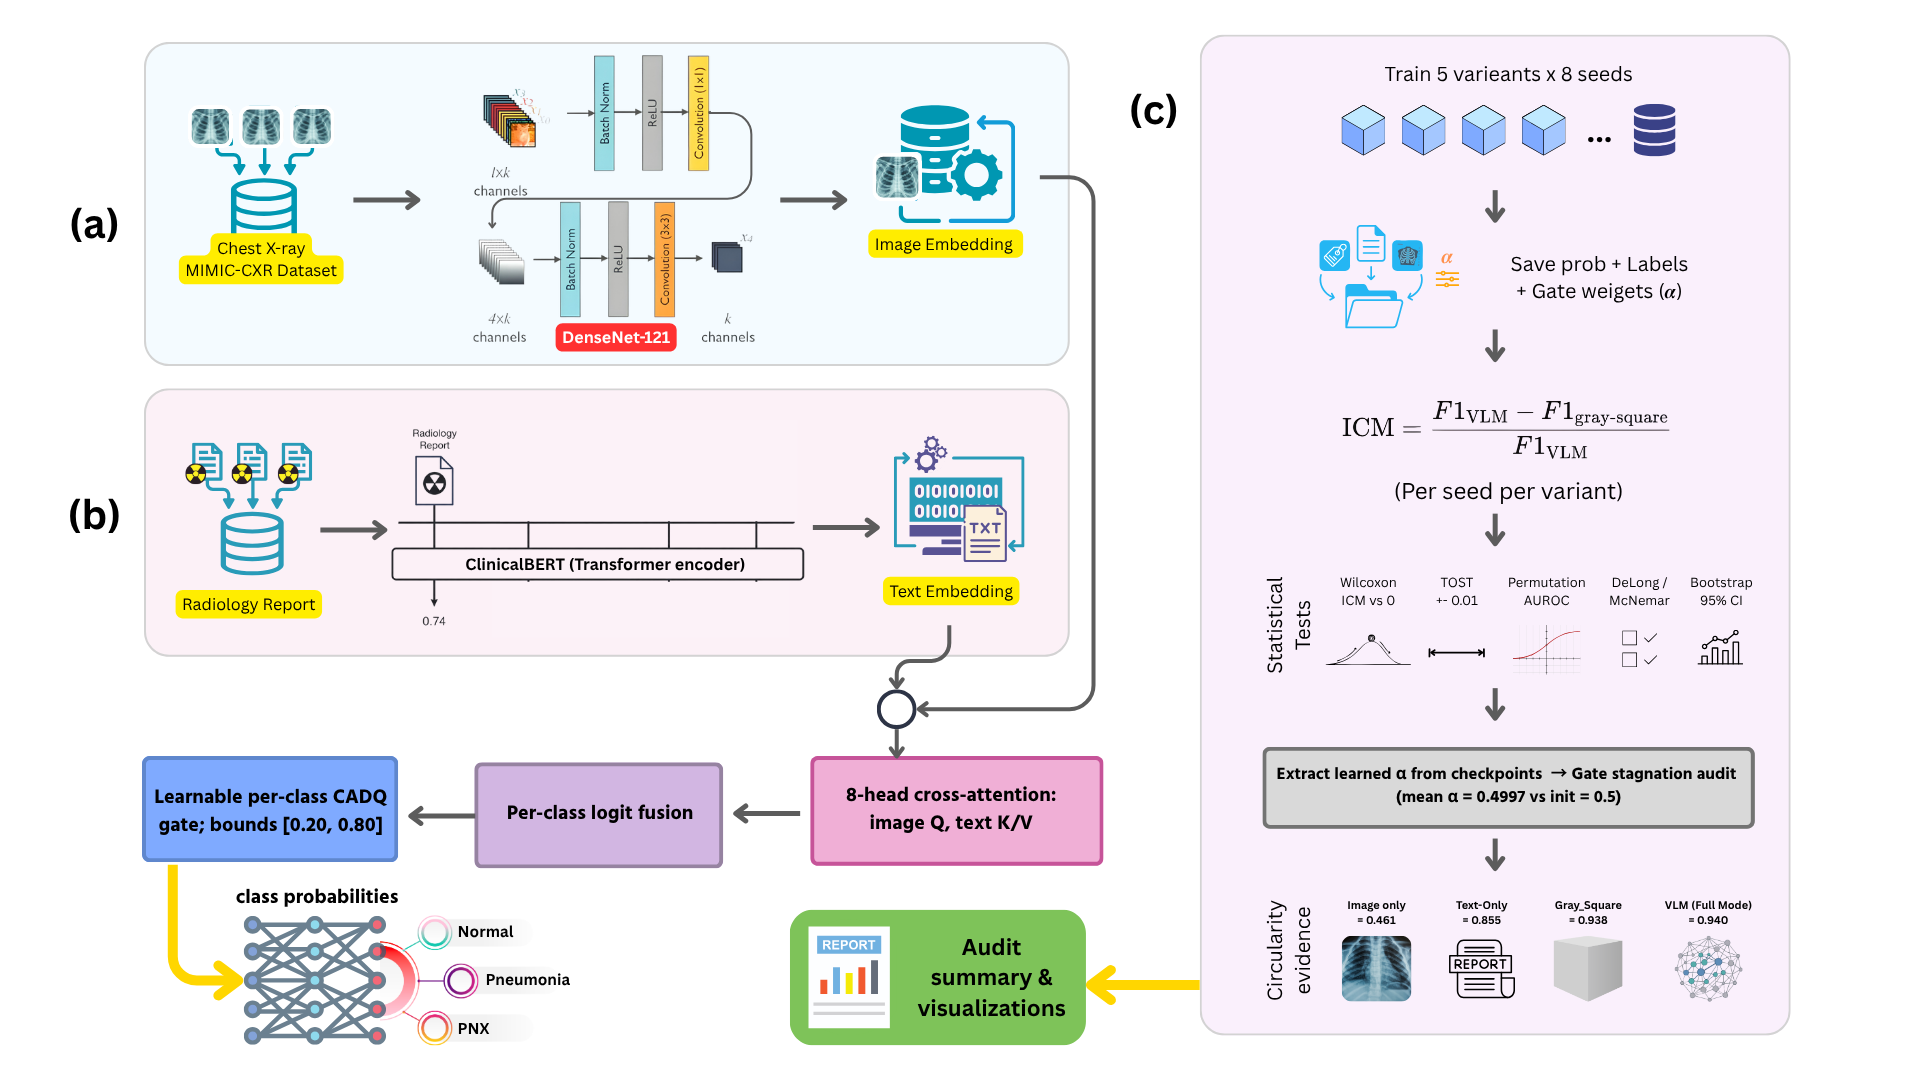
\includegraphics[width=0.94\textwidth]{methodology_diagram_v3_abc.png}
\caption{Image and report encoding, gated fusion, and seed-level modality audit.}
\label{fig:design}
\end{figure*}

Panel (a) summarizes DenseNet-121 image encoding, panel (b) shows the
Bio\_ClinicalBERT report pathway, and panel (c) links five eight-seed conditions
to ICM, statistical testing, gate extraction, and retained controls. Panel
identifiers are interpreted through this below-figure description rather than
as additional method claims. The diagram is not a layer-by-layer computational
graph: the retained model uses 512-dimensional projections, findings-only text,
separate class logits, and a static baseline gate. DeLong and McNemar use
retained seed-42 outputs, and each unimodal or Gray-Square control has one
retained run.

MIMIC-CXR JPG images and reports were accessed through official PhysioNet
credentialing under the applicable Data Use Agreement
\cite{johnson2019mimiccxr}. The source flow comprised 377,110 images in 227,835
studies; 227,827 studies had CheXpert labels and 108,626 met the frontal-view
eligibility criteria. An analysis cap selected up to 2,500 Normal, 2,500
Pneumonia, and 1,000 Pneumothorax candidates. Of 2,962 attempted downloads,
nine JPG files were unavailable, leaving 2,953 usable studies. The inherited
patient-level GroupShuffleSplit assigned 2,049 studies to training, 449 to
validation, and 455 to test, with no subject overlap. The test set contained
240 Normal, 168 Pneumonia, and 47 Pneumothorax studies.

The source counts were retained as a cohort ledger. The sequence was 377,110
images, 227,835 studies, 227,827 labelled studies, 108,626 eligible
frontal-view studies, 6,000 capped candidates, 2,962 download attempts, and
2,953 available studies. This accounting separates source-database size,
clinical eligibility, the practical analysis cap, and file availability. The
final class proportions should therefore be understood as properties of the
constructed audit cohort rather than prevalence estimates for MIMIC-CXR.

CheXpert generated the targets from report language using the project's
uncertain-to-negative mapping \cite{irvin2019chexpert}; the model received the
same report's \texttt{findings} field. The experiment consequently audits
label-report circularity rather than an independent radiograph-only diagnostic
task. The replication unit for seed-level inference was a trained model at a
fixed seed. Baseline CADQ, LearnedMixinFusion (LMH), noise-sensitivity
(anti-consistency), exploratory GACR-B, and Adaptive-CADQ each had eight
retained seeds: 42, 123, 456, 789, 1010, 1111, 1212, and 1313. The eight-seed
plan covered baseline, LMH, and noise-sensitivity (anti-consistency);
Adaptive-CADQ was extended from three to eight seeds after the initial run, and
exploratory GACR-B was added post hoc. The latter two analyses are
therefore exploratory.

Each study contributed one target to the three-class task. The patient-level
split was fixed before model evaluation so that images or reports from the same
person could not occur in more than one partition. This choice limits leakage
from repeated examinations that may share anatomy, wording patterns, or
clinical history. The same 455 test studies were reused across seeds and
conditions. This supports paired comparison, provided that repeated subjects
are not treated as independent observations when seed-level uncertainty is
estimated.

\subsection{Audit estimand and evidence hierarchy}\label{sec:estimand}

The audit is organized around a contrast rather than a model leaderboard. For
seed $s$, the observed full-model Macro-F1 is compared with the retained
Gray-Square Macro-F1 after spatial image information has been removed. The
report, target definition, class set, and held-out studies remain unchanged.
This contrast estimates how much the evaluated endpoint changes when the
declared image content is unavailable but the report-linked pathway remains.
It does not estimate the diagnostic value of chest radiography outside that
setting.

Evidence was interpreted in a fixed hierarchy. The report-preserving contrast
and ICM are primary because they directly intervene on image content. The
eight-seed distributions and paired tests quantify variation in the five
fusion conditions. Calibration, per-class sensitivity, and paired decision
counts are secondary because they show whether a similar average score hides a
change in confidence or error pattern. Gate extraction and Grad-CAM are
supporting observations: they can describe the retained model but cannot
replace an intervention.

This hierarchy guards against three common interpretation errors. First, the
text-only and image-only controls are not treated as symmetric estimates of
modality value because they use separate classifiers and only one retained run.
Second, a gate near 0.5 is not described as equal causal contribution from
image and text. Third, a non-significant difference from zero is not treated as
equivalence. The operational equivalence claim is made only through TOST and
only for the prespecified interval on the ICM scale.

The estimand is intentionally tied to Macro-F1. Let $F_{s}^{V}$ denote the
Macro-F1 of a full fusion condition at seed $s$, and let $F^{G}$ denote the
retained Gray-Square Macro-F1. The per-seed contrast is $F_{s}^{V}-F^{G}$, and
ICM divides that contrast by $F_{s}^{V}$. This normalization makes the value
easy to interpret relative to the full model, but it also means that ICM is
metric-specific. A near-zero Macro-F1 ICM does not imply near-zero change for
every class, threshold, or calibration measure; those quantities are examined
separately.

The label-report relationship is part of the estimand, not a nuisance removed
after analysis. CheXpert targets were derived from report language, and the
model received the corresponding findings text. The audit therefore asks how a
model behaves under that known information structure. It does not attempt to
reconstruct an unobserved independent radiologist label or to reinterpret the
report-derived target as image-only ground truth.

\subsection{Preprocessing and architecture}\label{sec:architecture}

The architecture exposes the contribution of each modality without changing
the downstream classification target. Image and report features were encoded
separately, projected to a common dimension, allowed to interact, and converted
to class-specific logits. The gate therefore combines class-level evidence
after feature extraction rather than deciding which raw input should be
retained.

The \texttt{findings} field was tokenized with
\texttt{emilyalsentzer/Bio\_ClinicalBERT}, truncated or padded to 256 tokens,
and randomly replaced by an empty string in 10\% of training examples. Test and
validation text was not masked. Images were converted to one channel, resized
to $256\times256$, randomly cropped to $224\times224$ during training, and
mapped from $[0,255]$ to $[-1,1]$. Training augmentation used horizontal
flipping, rotation up to $10^{\circ}$, translation, and brightness/contrast
jitter; the minority-class transform increased the rotation, translation,
scale, shear, jitter, and blur ranges. Validation and test preprocessing was
deterministic. Residual non-uniform effects of this mapping cannot be fully
excluded; it is treated as a shared preprocessing constraint across all
conditions \cite{cohen2022torchxrayvision}.

The stronger minority-class augmentation was applied only during training. It
was intended to increase variation for the rarer classes without changing
validation or test inputs. No transformation used test labels or test-set
statistics. All image-bearing fusion conditions used the same transform family
and fixed split, so a cross-condition difference was not coupled to a separate
evaluation pipeline.

The image branch used a TorchXRayVision DenseNet-121 with
\texttt{densenet121-res224-mimic\_ch} weights
\cite{huang2017densenet,cohen2022torchxrayvision}. All image-bearing fusion
conditions shared the same $[-1,1]$ intensity mapping. Any deviation from the
native TorchXRayVision convention therefore acts as a shared preprocessing
shift across conditions. ICM and condition contrasts characterize the retained
preprocessing setting.
The encoder's convolutional stem and
first dense block were frozen, and its output was projected to 512 dimensions
through a linear layer, LayerNorm, Gaussian Error Linear Unit, and dropout
(0.25). The text branch used Bio\_ClinicalBERT with the first four transformer
layers frozen and an analogous 512-dimensional projection
\cite{devlin2019bert,alsentzer2019clinicalbert}. One projected image token was
used as the query and one projected text token as the key/value in an eight-head
attention block with residual LayerNorm. Because there is only one key, this
operation cannot express word-region alignment; we interpret it as feature
interaction, not causal attention.

The single image token and single text token create a compact fusion interface,
but they also restrict what attention can represent. The attention output can
mix projected modality features; it cannot resolve individual report tokens
against spatial image regions. This boundary is carried into the interpretation
of the qualitative saliency examples. The architecture permits a test of image
sensitivity, but it does not support claims about phrase-level anatomical
alignment.

Baseline CADQ combined image and text logits through a bounded learnable
per-class gate \cite{arevalo2017gmu}:
\begin{equation}
\begin{aligned}
\alpha_c&=0.20+0.60\operatorname{sigmoid}(u_c),\\
z_c&=\alpha_c z^{\mathrm{img}}_c+(1-\alpha_c)z^{\mathrm{text}}_c.
\end{aligned}
\end{equation}
The initial logits $u=(-0.5,0,0.5)$ corresponded to image-gate values
$(0.426524,0.500000,0.573476)$ for Normal, Pneumonia, and Pneumothorax.

\subsection{Experimental conditions and modality controls}\label{sec:conditions}

The experimental design changes one aspect of fusion or regularization at a
time while preserving the cohort and three-class endpoint. Baseline CADQ is the
reference. LMH tests a learned text-prior correction, the noise-sensitivity
(anti-consistency) condition tests response to perturbed images, exploratory
GACR-B adds a grounding-aware penalty, and Adaptive-CADQ changes the gate from
static to input-dependent. Table~\ref{tab:conditions} records the intended
contrast and the evidence boundary for each condition.

LMH added a five-fold out-of-fold term-frequency/inverse-document-frequency
logistic text prior (5,000 unigram/bigram features, stop-word removal, balanced
weights), temperature calibration, $\epsilon=0.1$ smoothing, an input-dependent
prior gate, and an entropy penalty of 0.05 annealed over three epochs. It was
warm-started from CADQ and followed the product-of-experts rationale used for
unimodal-bias reduction \cite{cadene2019rubi}. The noise-sensitivity
(anti-consistency) condition perturbed the
image with Gaussian noise ($\sigma=0.25$). Its archived objective added
$-D_{KL}(p_{clean}\|p_{noisy})$ to a minimized loss and therefore rewards
divergence; throughout this manuscript it is treated as a noise-sensitivity
(anti-consistency) condition, not a conventional consistency objective.
Adaptive-CADQ replaced the static per-class gate with a sample-dependent scalar
computed from image and text entropies by a $2\rightarrow16\rightarrow1$
multilayer perceptron. Exploratory GACR-B used an out-of-fold text baseline and
a cosine penalty of 0.3 on examples for which that baseline misclassified, following
the grounding-aware intervention of Sadanandan and Behzadan
\cite{sadanandan2026consistentdangerous}.

The image-only control used the image encoder with a 512-to-256 classifier; the
text-only control used frozen Bio\_ClinicalBERT with a 768-to-256 classifier.
The Gray-Square control replaced every image by a constant intensity-128 tensor
but preserved the report and multimodal architecture. Only one retained run was
available for each control. Gray-Square is therefore a report-preserving image
ablation, not an independently trained eight-seed text-only ensemble.

The three controls answer different questions. Image-only and text-only models
describe the capacity of isolated pathways under their retained training
configurations. Gray-Square preserves the multimodal path while removing
spatially varying image content. It is the primary comparator because the
report, target, architecture, and evaluation cohort remain fixed. The
single-run control coverage is reported explicitly so that its unmeasured
run-to-run uncertainty is not confused with the eight-seed variation of the
fusion conditions.

\begin{table*}[t]
\centering
\caption{Experimental conditions and their audit roles.}
\label{tab:conditions}
\small
\setlength{\tabcolsep}{4pt}
\resizebox{0.99\textwidth}{!}{%
\begin{tabular}{p{0.17\textwidth}p{0.25\textwidth}p{0.25\textwidth}p{0.25\textwidth}}
\toprule
Condition & Change from baseline & Question addressed & Interpretation boundary \\
\midrule
Baseline CADQ & Static bounded per-class gate & Reference performance and image-replacement sensitivity & Gate value is not a causal contribution estimate. \\
LMH (PoE) & Learned text prior and product-of-experts correction & Does reducing the easy text route increase image contribution? & A lower score can reflect removal of target-linked report information. \\
Noise-sensitivity (anti-consistency) & Gaussian image perturbation with the retained negative-KL term & How does the archived objective respond to image noise? & The loss rewards divergence and is not conventional consistency training. \\
Exploratory GACR-B & Text-baseline-aware cosine penalty & Does a grounding-aware intervention alter contribution? & Added post hoc and interpreted as exploratory. \\
Adaptive-CADQ & Entropy-conditioned dynamic gate & Does input-dependent gating improve reliance over a static gate? & Dynamic weight variation does not by itself establish grounding. \\
Gray-Square & Constant image with report and multimodal path retained & Primary report-preserving image ablation & One retained run; comparator variance is not independently estimated. \\
Text-only and image-only & Separate unimodal classifiers & Descriptive capacity of each isolated pathway & Different retained control pipelines prevent a definitive modality ranking. \\
\bottomrule
\end{tabular}}
\end{table*}

\subsection{Training and outcomes}\label{sec:training}

Training was held constant wherever the retained experiment allowed so that
changes could be attributed to the tested condition rather than a separate
optimization schedule. Model selection used validation Macro-F1 for the five
multimodal conditions. Test metrics were computed after training and checkpoint
selection; the held-out test set was not used to tune hyperparameters, select
thresholds, or define the operational equivalence interval.

Models were trained for 10 epochs with AdamW and weight decay $10^{-4}$
\cite{loshchilov2019adamw}. Learning rates were $10^{-5}$ for the image and text
backbones, $10^{-4}$ for fusion and LMH heads, and $5\times10^{-5}$ for static
gates. OneCycleLR used 10\% warm-up \cite{smith2019superconvergence}. Physical
batch size was 8 with four gradient-accumulation steps (effective batch 32),
mixed precision, and gradient scaling. The objective combined focal
cross-entropy ($\gamma=1.5$), label smoothing (0.05), and effective-number class
weights ($\beta=0.99$) \cite{lin2017focalloss}. Class-aware sampling replicated
Pneumothorax examples up to fivefold and Pneumonia examples up to threefold.
The highest validation Macro-F1 checkpoint was restored for multimodal
conditions. The image-only control was retained as a descriptive capacity
probe; its archived pipeline did not guarantee restoration of the best
validation checkpoint. Inferential claims about modality reliance rest on the
report-preserving Gray-Square intervention, not the image-only result.

Class-aware sampling changed the frequency with which examples were presented
during optimization but did not change the held-out class distribution. The
reported test metrics therefore describe the fixed 455-study test cohort rather
than the sampling distribution used to construct mini-batches. Mixed precision
and gradient accumulation were computational choices shared across conditions;
they are recorded because small parameter movements, including gate drift, must
be interpreted in the numerical setting in which checkpoints were saved.

Validation Macro-F1 aligned checkpoint selection with the primary performance
scale while preserving the test set for final evaluation. The multimodal
conditions used the best retained validation checkpoint. The image-only control
is kept as a capacity probe because its archived selection path did not provide
the same guarantee. This asymmetry is why the image-only number is not used in
ICM and why the report-preserving Gray-Square contrast anchors the main
inference.

The primary diagnostic was
\begin{equation}
\mathrm{ICM}=\frac{F1_{VLM}-F1_{Gray}}{F1_{VLM}},
\end{equation}
where positive values indicate better Macro-F1 with the real radiograph. The
relative form was chosen to express the incremental change on the scale of the
full model. An ICM near zero indicates that replacing the image did not
materially change this endpoint; it does not prove that the image encoder is
universally uninformative. The analysis used an operational equivalence interval
of $[-0.01,0.01]$. This project-defined margin is neither a validated clinical
threshold nor a regulatory acceptance criterion.

ICM is signed. A positive value means the full model achieved higher Macro-F1
than the Gray-Square reference; a negative value means the retained reference
was higher. The denominator expresses the change relative to the full-model
score. We report the absolute Macro-F1 values beside ICM so that the normalized
quantity cannot hide a small denominator or an otherwise poorly performing
model. In this experiment the full-model scores are near 0.94, so absolute and
relative differences are both readily interpretable.

Secondary outcomes were Macro-F1, accuracy, one-versus-rest Macro-AUROC,
per-class F1 and sensitivity, ten-bin expected calibration error (ECE),
multiclass Brier score, row-normalized confusion matrices, retained image-gate
values, and qualitative Grad-CAM. ECE and Brier were recomputed from retained
probability arrays when absent from the summary dictionary; missing values were
never replaced with zero. Gate values were taken from the per-seed checkpoint
export in \texttt{q1\_audit\_results.json}. The displayed gate figure uses all
eight exported values and their equation-derived initialization references,
rather than hard-coded aggregate values.

Macro-F1 was primary because the three classes were imbalanced and the rare
Pneumothorax class should not be hidden by the larger Normal group. Accuracy and
Macro-AUROC describe complementary aspects of prediction but cannot alone show
whether a model uses the image. ECE and Brier score were included because two
conditions can rank cases similarly while assigning materially different
confidence. Per-class sensitivity and confusion matrices localize changes that
an average metric can conceal.

Gate extraction was defined as a parameter audit rather than an attribution
method. For every baseline seed, the saved checkpoint value was transformed by
the same bounded sigmoid equation used during inference and compared with its
class-specific initialization. We use the term \emph{gate stagnation} for the
observed pattern of negligible movement. The label describes parameter
stability only; it does not establish that gradients were zero or identify the
cause of that stability.

\subsection{Statistical analysis and reproducibility}\label{sec:statistics}

The statistical plan separates three questions. Paired tests assess whether a
condition differs from baseline, equivalence tests assess whether ICM lies
inside the operational near-zero interval, and bootstrap intervals summarize
uncertainty across retained seeds. Subject-level tests were limited to matched
seed-42 arrays because probability and prediction files for all comparable
seeds were not uniformly available.

Seed-level differences used paired Wilcoxon signed-rank tests with Pratt zero
handling and paired $t$-tests. ICM summaries included the median, standard
deviation, Cohen's $d$, and percentile bootstrap 95\% confidence intervals from
2,000 resamples. Two one-sided tests (TOST) evaluated whether ICM lay within
$[-0.01,0.01]$ \cite{lakens2017equivalence}. Because the same 455 studies recur
at every seed, test subjects were not concatenated across seeds for
confirmatory inference.

DeLong tests compared correlated Pneumothorax receiver-operating-characteristic
curves within the retained seed-42 probability set \cite{delong1988roc}.
McNemar tests compared paired classification decisions on the same 455 seed-42
studies \cite{mcnemar1947correlated}. Benjamini-Hochberg correction controlled
the false-discovery rate within each test family
\cite{benjamini1995fdr}. A McNemar $p$-value of 1 denotes balanced discordance,
not identical predictions; the two off-diagonal counts are therefore reported
with the test result.

Python, NumPy, and PyTorch seeds were fixed and deterministic cuDNN settings
were enabled. Run metadata, validation histories, checkpoints, predictions,
probabilities, and configurations were retained. The fixed merge archive
resolved duplicate keys by the first-seen value, but the earlier workflow did
not preserve a deterministic source-priority rule and content-hash manifest.
Results are consequently tied to this archive snapshot. Reporting was audited
against CLAIM and TRIPOD+AI principles
\cite{mongan2024claim,collins2024tripodai}; checklist summaries and a provenance
manifest are included in the Supplementary material.

Analyses were performed on fixed retained outputs rather than by pooling
predictions from separate seeds into a larger artificial sample. This preserves
the trained model as the replication unit for seed-level comparisons. It also
avoids confidence intervals that would appear too narrow because the same 455
patients recur under every seed. All inferential results are reported with the
test family, unit of analysis, and multiplicity adjustment needed to interpret
them.

\section{Results}\label{sec:results}

Results are presented in the order needed to evaluate the modality claim. We
first describe predictive performance across the five eight-seed conditions,
then examine paired tests and calibration. The report-preserving Gray-Square
comparison provides the primary evidence for incremental image contribution.
Gate extraction and qualitative saliency are reported last because they support
interpretation but do not independently establish modality use.

\subsection{Analysis set, discrimination, and calibration}\label{sec:performance}

The fixed archive contained 40 condition-seed records: five conditions with
eight seeds each, evaluated on the same 455 held-out studies. Baseline CADQ
achieved Macro-F1 $0.9397\pm0.0061$, accuracy $0.9607\pm0.0032$, and
Macro-AUROC $0.9974\pm0.0004$ (Table~\ref{tab:performance}). LMH had the
highest mean Macro-F1 ($0.9435\pm0.0093$) but lower and more variable AUROC
($0.9849\pm0.0113$). The noise-sensitivity (anti-consistency) condition had
the lowest Macro-F1 ($0.9346\pm0.0075$). Exploratory GACR-B reached
$0.9417\pm0.0059$, and
Adaptive-CADQ remained close to baseline at $0.9388\pm0.0072$.

The narrow range of mean Macro-F1 values shows that the five optimization
strategies reached similar aggregate endpoints. The ranking alone is not
sufficient to identify an improvement: the largest mean belongs to LMH, but its
seed variability is wider and its calibration and AUROC move in the opposite
direction. The baseline therefore remains the reference for the modality audit
rather than being replaced by the condition with the highest unadjusted mean.

\begin{table*}[t]
\centering
\caption{Performance and calibration across eight seeds.}
\label{tab:performance}
\scriptsize
\setlength{\tabcolsep}{3.2pt}
\resizebox{0.94\textwidth}{!}{%
\begin{tabular}{lccccc}
\toprule
Condition & Macro-F1 & Accuracy & Macro-AUROC & ECE & Brier \\
\midrule
Baseline CADQ & $0.9397\pm0.0061$ & $0.9607\pm0.0032$ & $0.9974\pm0.0004$ & $0.0237\pm0.0048$ & $0.0522\pm0.0040$ \\
LMH (PoE) & $0.9435\pm0.0093$ & $0.9596\pm0.0070$ & $0.9849\pm0.0113$ & $0.0621\pm0.0160$ & $0.0685\pm0.0213$ \\
Noise-sensitivity (anti-consistency) & $0.9346\pm0.0075$ & $0.9560\pm0.0039$ & $0.9960\pm0.0013$ & $0.0347\pm0.0137$ & $0.0655\pm0.0130$ \\
Exploratory GACR-B & $0.9417\pm0.0059$ & $0.9610\pm0.0042$ & $0.9972\pm0.0005$ & $0.0245\pm0.0023$ & $0.0540\pm0.0038$ \\
Adaptive-CADQ & $0.9388\pm0.0072$ & $0.9610\pm0.0044$ & $0.9972\pm0.0008$ & $0.0241\pm0.0070$ & $0.0527\pm0.0028$ \\
\bottomrule
\end{tabular}}
\end{table*}

The multiplicity-adjusted tests did not identify a Macro-F1 improvement over
baseline. At seed 42, LMH and the noise-sensitivity (anti-consistency) condition
produced measurable AUROC degradation even though their absolute AUROC values
remained high. This combination illustrates why ceiling-level discrimination
can hide a directional loss. The McNemar results add a separate view: they test
whether paired errors changed direction, not whether two prediction vectors are
identical.

Baseline per-class F1 was $0.9755\pm0.0032$ for Normal,
$0.9624\pm0.0055$ for Pneumonia, and $0.8810\pm0.0174$ for
Pneumothorax. LMH increased Pneumothorax F1 to $0.9003\pm0.0191$ but
reduced Pneumonia F1 to $0.9575\pm0.0077$. The noise-sensitivity
(anti-consistency) condition had the
widest Pneumothorax variation ($0.8753\pm0.0237$). Adaptive-CADQ showed
the most stable Pneumonia F1 ($0.9616\pm0.0029$). The distributions and
retained controls are shown in Fig.~\ref{fig:performance-controls}. The control
panel is not an accuracy ranking across equally replicated systems: each
control represents one retained run, whereas each fusion distribution contains
eight seeds.

\begin{figure*}[t]
\centering
\begin{minipage}[t]{0.57\textwidth}
\centering
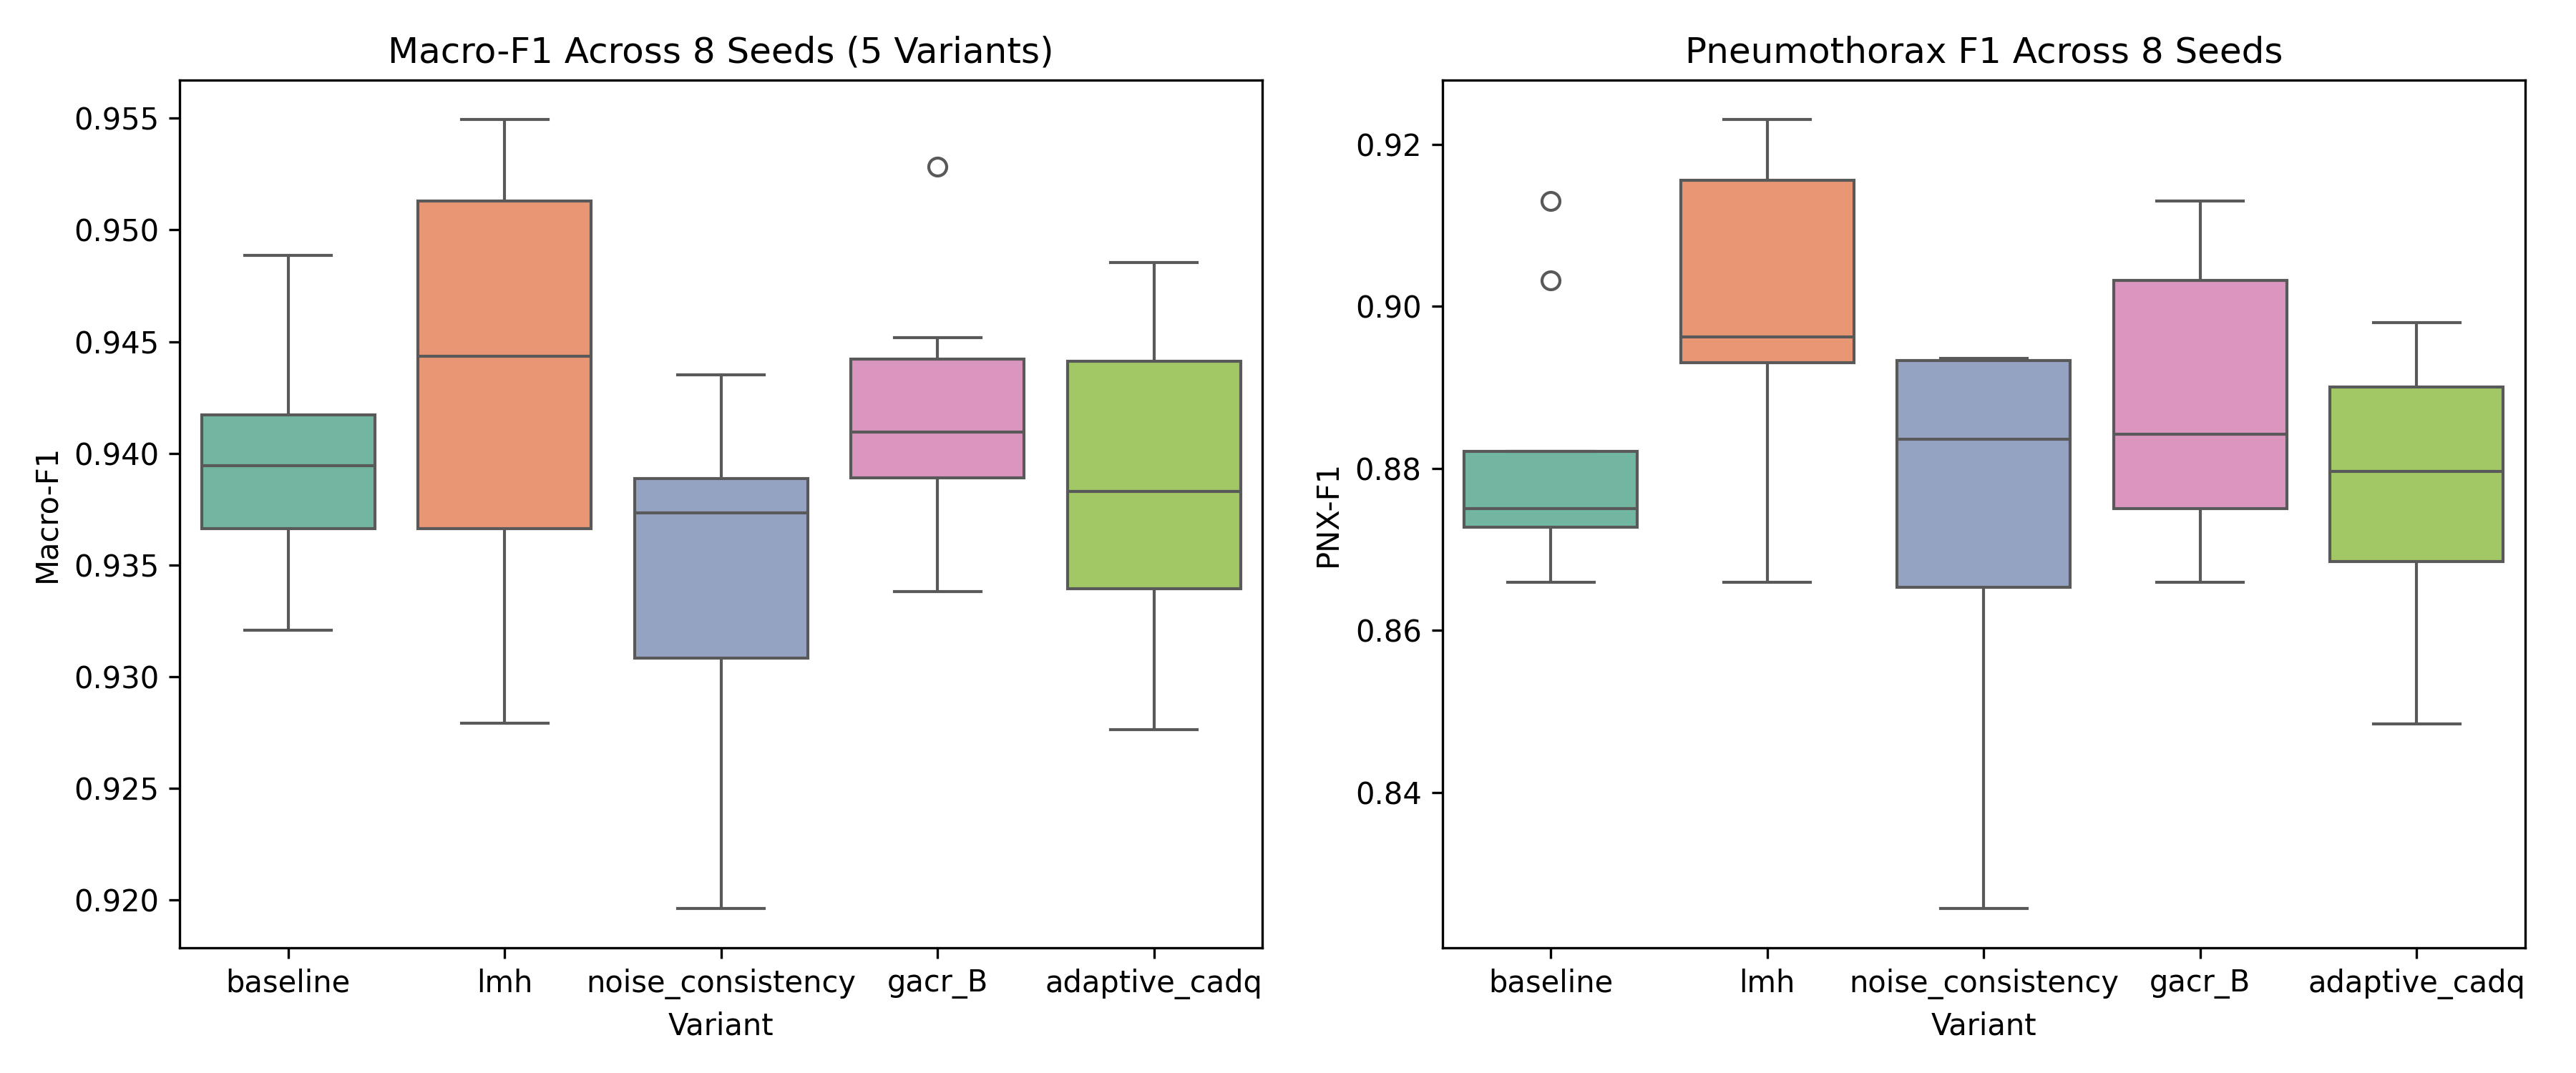
\includegraphics[width=\linewidth]{f1_boxplots.png}\par
\textbf{(a)}
\end{minipage}\hfill
\begin{minipage}[t]{0.38\textwidth}
\centering
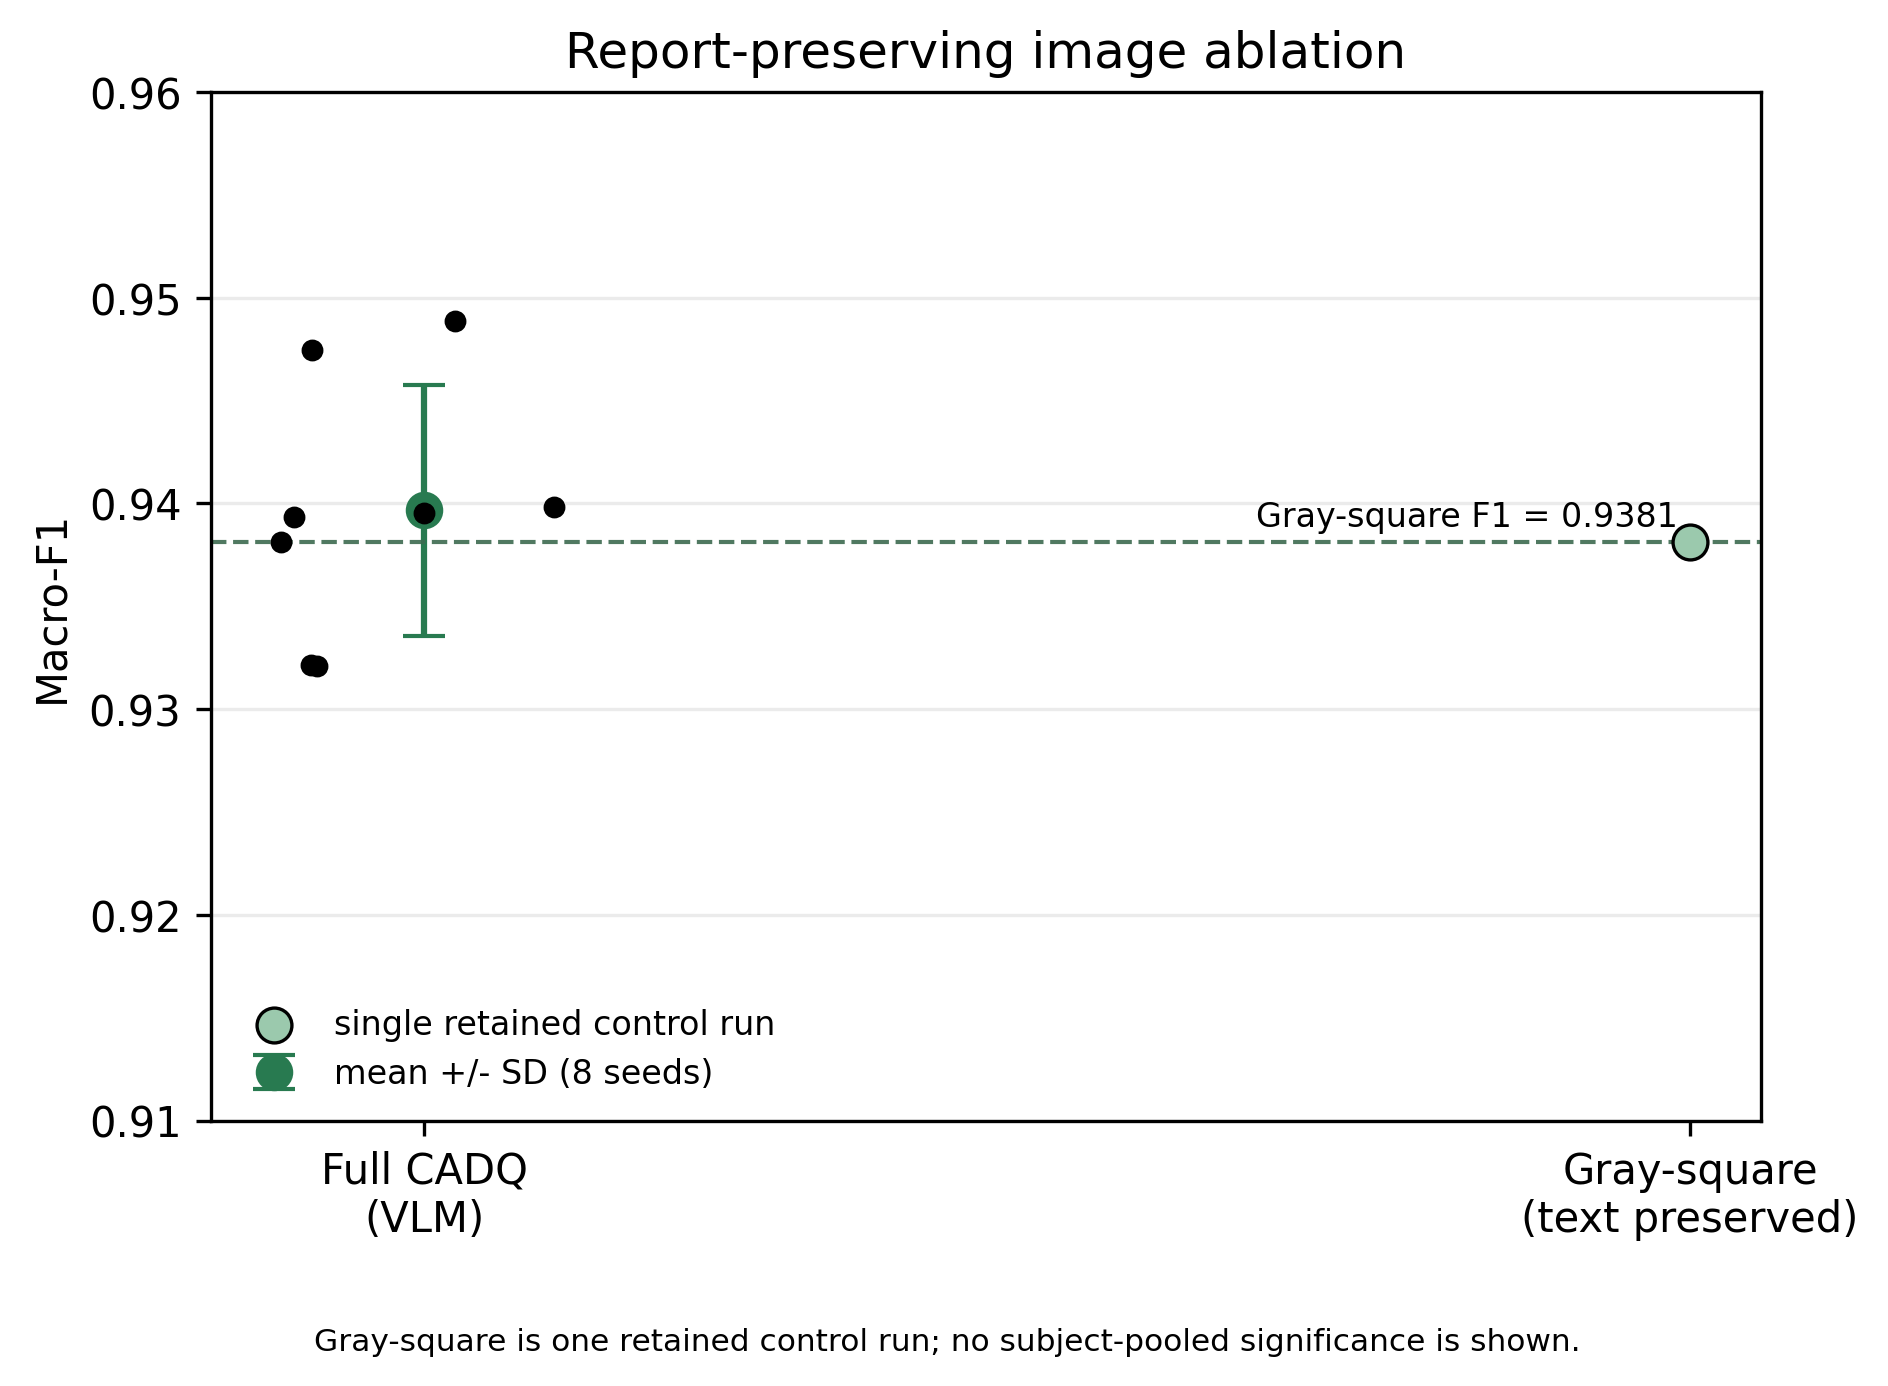
\includegraphics[width=0.82\linewidth]{circularity_contrast.png}\par
\textbf{(b)}
\end{minipage}
\caption{Fusion-condition F1 distributions and retained modality controls.}
\label{fig:performance-controls}
\end{figure*}

No condition improved Macro-F1 over baseline after Benjamini-Hochberg
correction (Table~\ref{tab:pairwise}). The largest unadjusted Macro-F1 signal
was the exploratory GACR-B contrast ($\Delta=0.0020$, Wilcoxon $p=0.0547$;
adjusted $p=0.2188$). LMH and the noise-sensitivity (anti-consistency)
condition had lower seed-42
Pneumothorax AUROC than baseline; their significant DeLong results indicate
degradation, not improvement. Adaptive-CADQ showed no AUROC difference.

Table~\ref{tab:pairwise} uses eight paired seed-level Macro-F1 values for the
Wilcoxon comparisons. DeLong and McNemar use the retained seed-42 probability
and prediction arrays for the same 455 studies. Parenthetical values are
Benjamini-Hochberg adjusted within each test family, and $n_{01}/n_{10}$ are the
two McNemar discordant counts.

\begin{table*}[t]
\centering
\caption{Paired comparisons with the baseline condition.}
\label{tab:pairwise}
\scriptsize
\resizebox{0.96\textwidth}{!}{%
\begin{tabular}{lccc}
\toprule
Condition & Wilcoxon Macro-F1 $p$ (BH) & DeLong PNX-AUROC $p$ (BH) & McNemar $n_{01}/n_{10}$; $p$ (BH) \\
\midrule
LMH (PoE) & 0.2500 (0.3333) & $2.9\times10^{-6}$ ($1.2\times10^{-5}$) & 27/31; 0.6936 (1.0000) \\
Noise-sensitivity (anti-consistency) & 0.1953 (0.3333) & 0.0022 (0.0044) & 32/49; 0.0754 (0.3018) \\
Exploratory GACR-B & 0.0547 (0.2188) & 0.0315 (0.0420) & 9/8; 1.0000 (1.0000) \\
Adaptive-CADQ & 0.8438 (0.8438) & 0.7304 (0.7304) & 15/14; 1.0000 (1.0000) \\
\bottomrule
\end{tabular}}
\end{table*}

The balanced discordance for exploratory GACR-B and Adaptive-CADQ is informative.
Exploratory GACR-B disagreed
with baseline on 17 studies (9 versus 8 across the two off-diagonal directions),
and Adaptive-CADQ on 29 (15 versus 14). McNemar $p=1.000$ indicates no evidence
of directional asymmetry in these paired errors; it does not indicate
byte-identical predictions. The confusion matrices and receiver-operating-
characteristic curves in Fig.~\ref{fig:error-roc} are descriptive views of the
same repeated test cohort. The confusion matrices are row-normalized and
aggregated over seeds. The ROC bands summarize multi-seed variation, whereas
DeLong inference uses matched seed-42 arrays and was not performed on subjects
pooled across seeds. Significant DeLong results for LMH, the
noise-sensitivity (anti-consistency) condition, and exploratory GACR-B indicate
lower Pneumothorax AUROC than baseline rather than improvement.

\begin{figure*}[t]
\centering
\begin{minipage}[t]{0.52\textwidth}
\centering
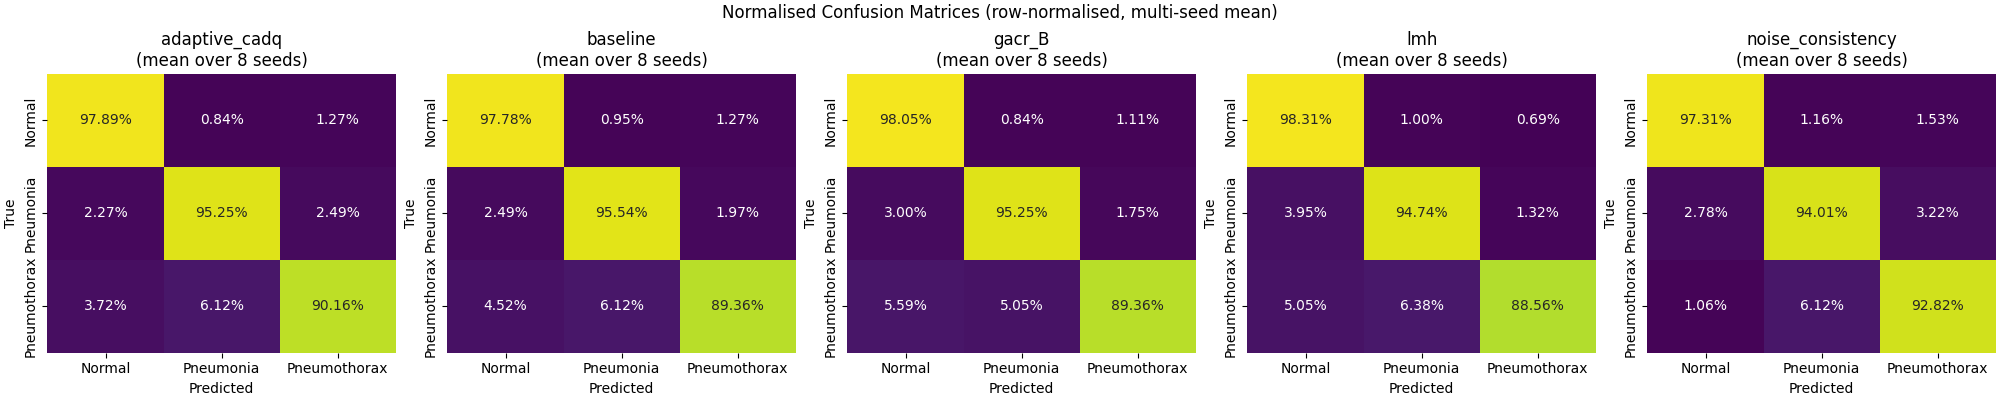
\includegraphics[width=\linewidth]{confusion_matrices_normalised.png}\par
\textbf{(a)}
\end{minipage}\hfill
\begin{minipage}[t]{0.43\textwidth}
\centering
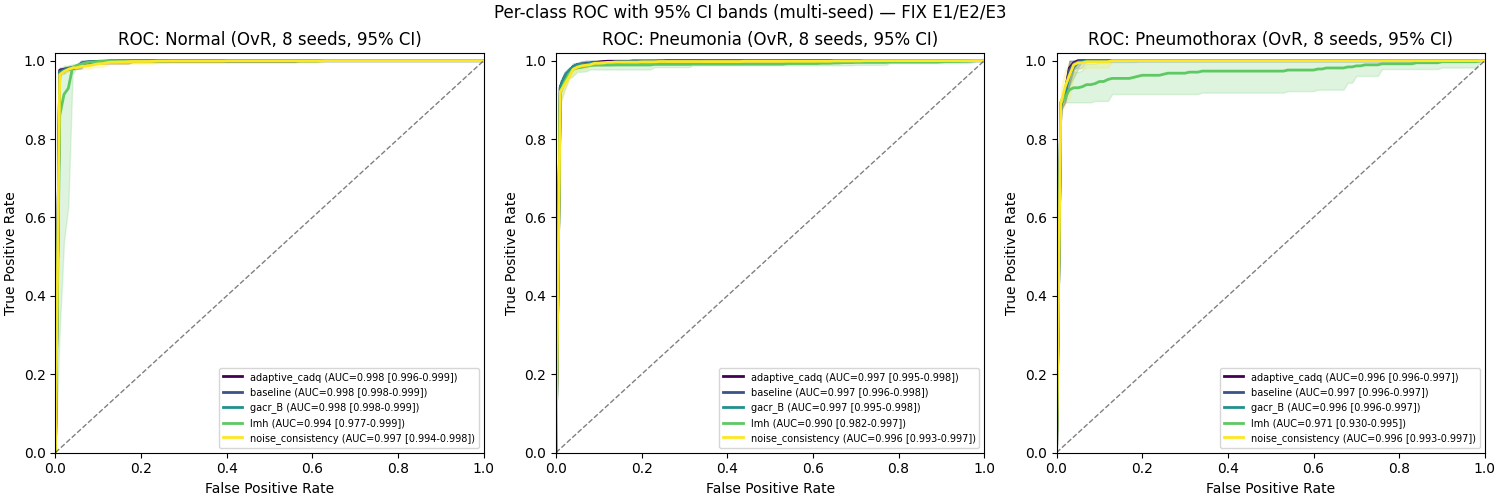
\includegraphics[width=\linewidth]{roc_curves_with_ci.png}\par
\textbf{(b)}
\end{minipage}
\caption{Row-normalized confusion matrices and class-specific ROC curves.}
\label{fig:error-roc}
\end{figure*}

Calibration separated some conditions that had similar Macro-F1. Baseline ECE
was $0.0237\pm0.0048$ and Brier score $0.0522\pm0.0040$. LMH increased ECE
to $0.0621\pm0.0160$ (2.6-fold) and Brier score to
$0.0685\pm0.0213$; the adjusted seed-level $p$-values were 0.0313 and 0.0156.
The noise-sensitivity (anti-consistency) condition increased Brier score to
$0.0655\pm0.0130$ (adjusted $p=0.0156$), whereas its ECE change was
inconclusive. Exploratory GACR-B and
Adaptive-CADQ remained close to baseline. Figure~\ref{fig:calibration} shows
the baseline reliability diagram and seed-level ECE distributions.

The reliability panel is descriptive and uses confidence bins to compare
observed correctness with predicted confidence. The seed-level ECE panel shows
the dispersion hidden by a single mean. Together they indicate that LMH's small
Macro-F1 difference did not represent a uniformly better model: confidence
quality deteriorated while classification performance remained close to the
baseline range.

\begin{figure*}[t]
\centering
\begin{minipage}[t]{0.42\textwidth}
\centering
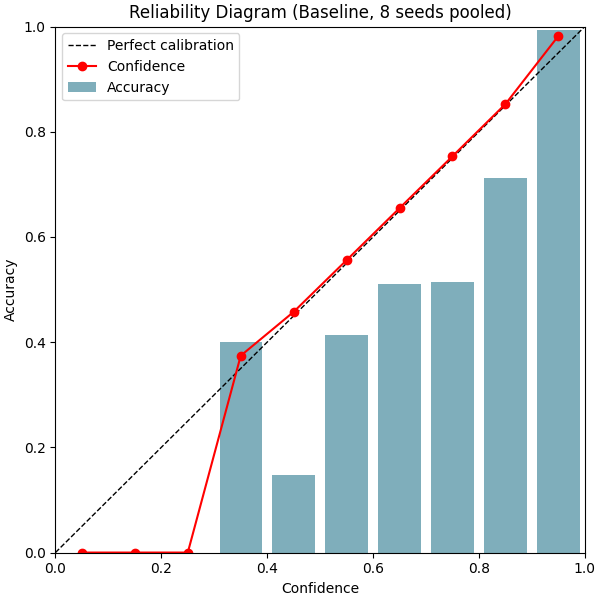
\includegraphics[width=\linewidth]{reliability_diagram.png}\par
\textbf{(a)}
\end{minipage}\hfill
\begin{minipage}[t]{0.53\textwidth}
\centering
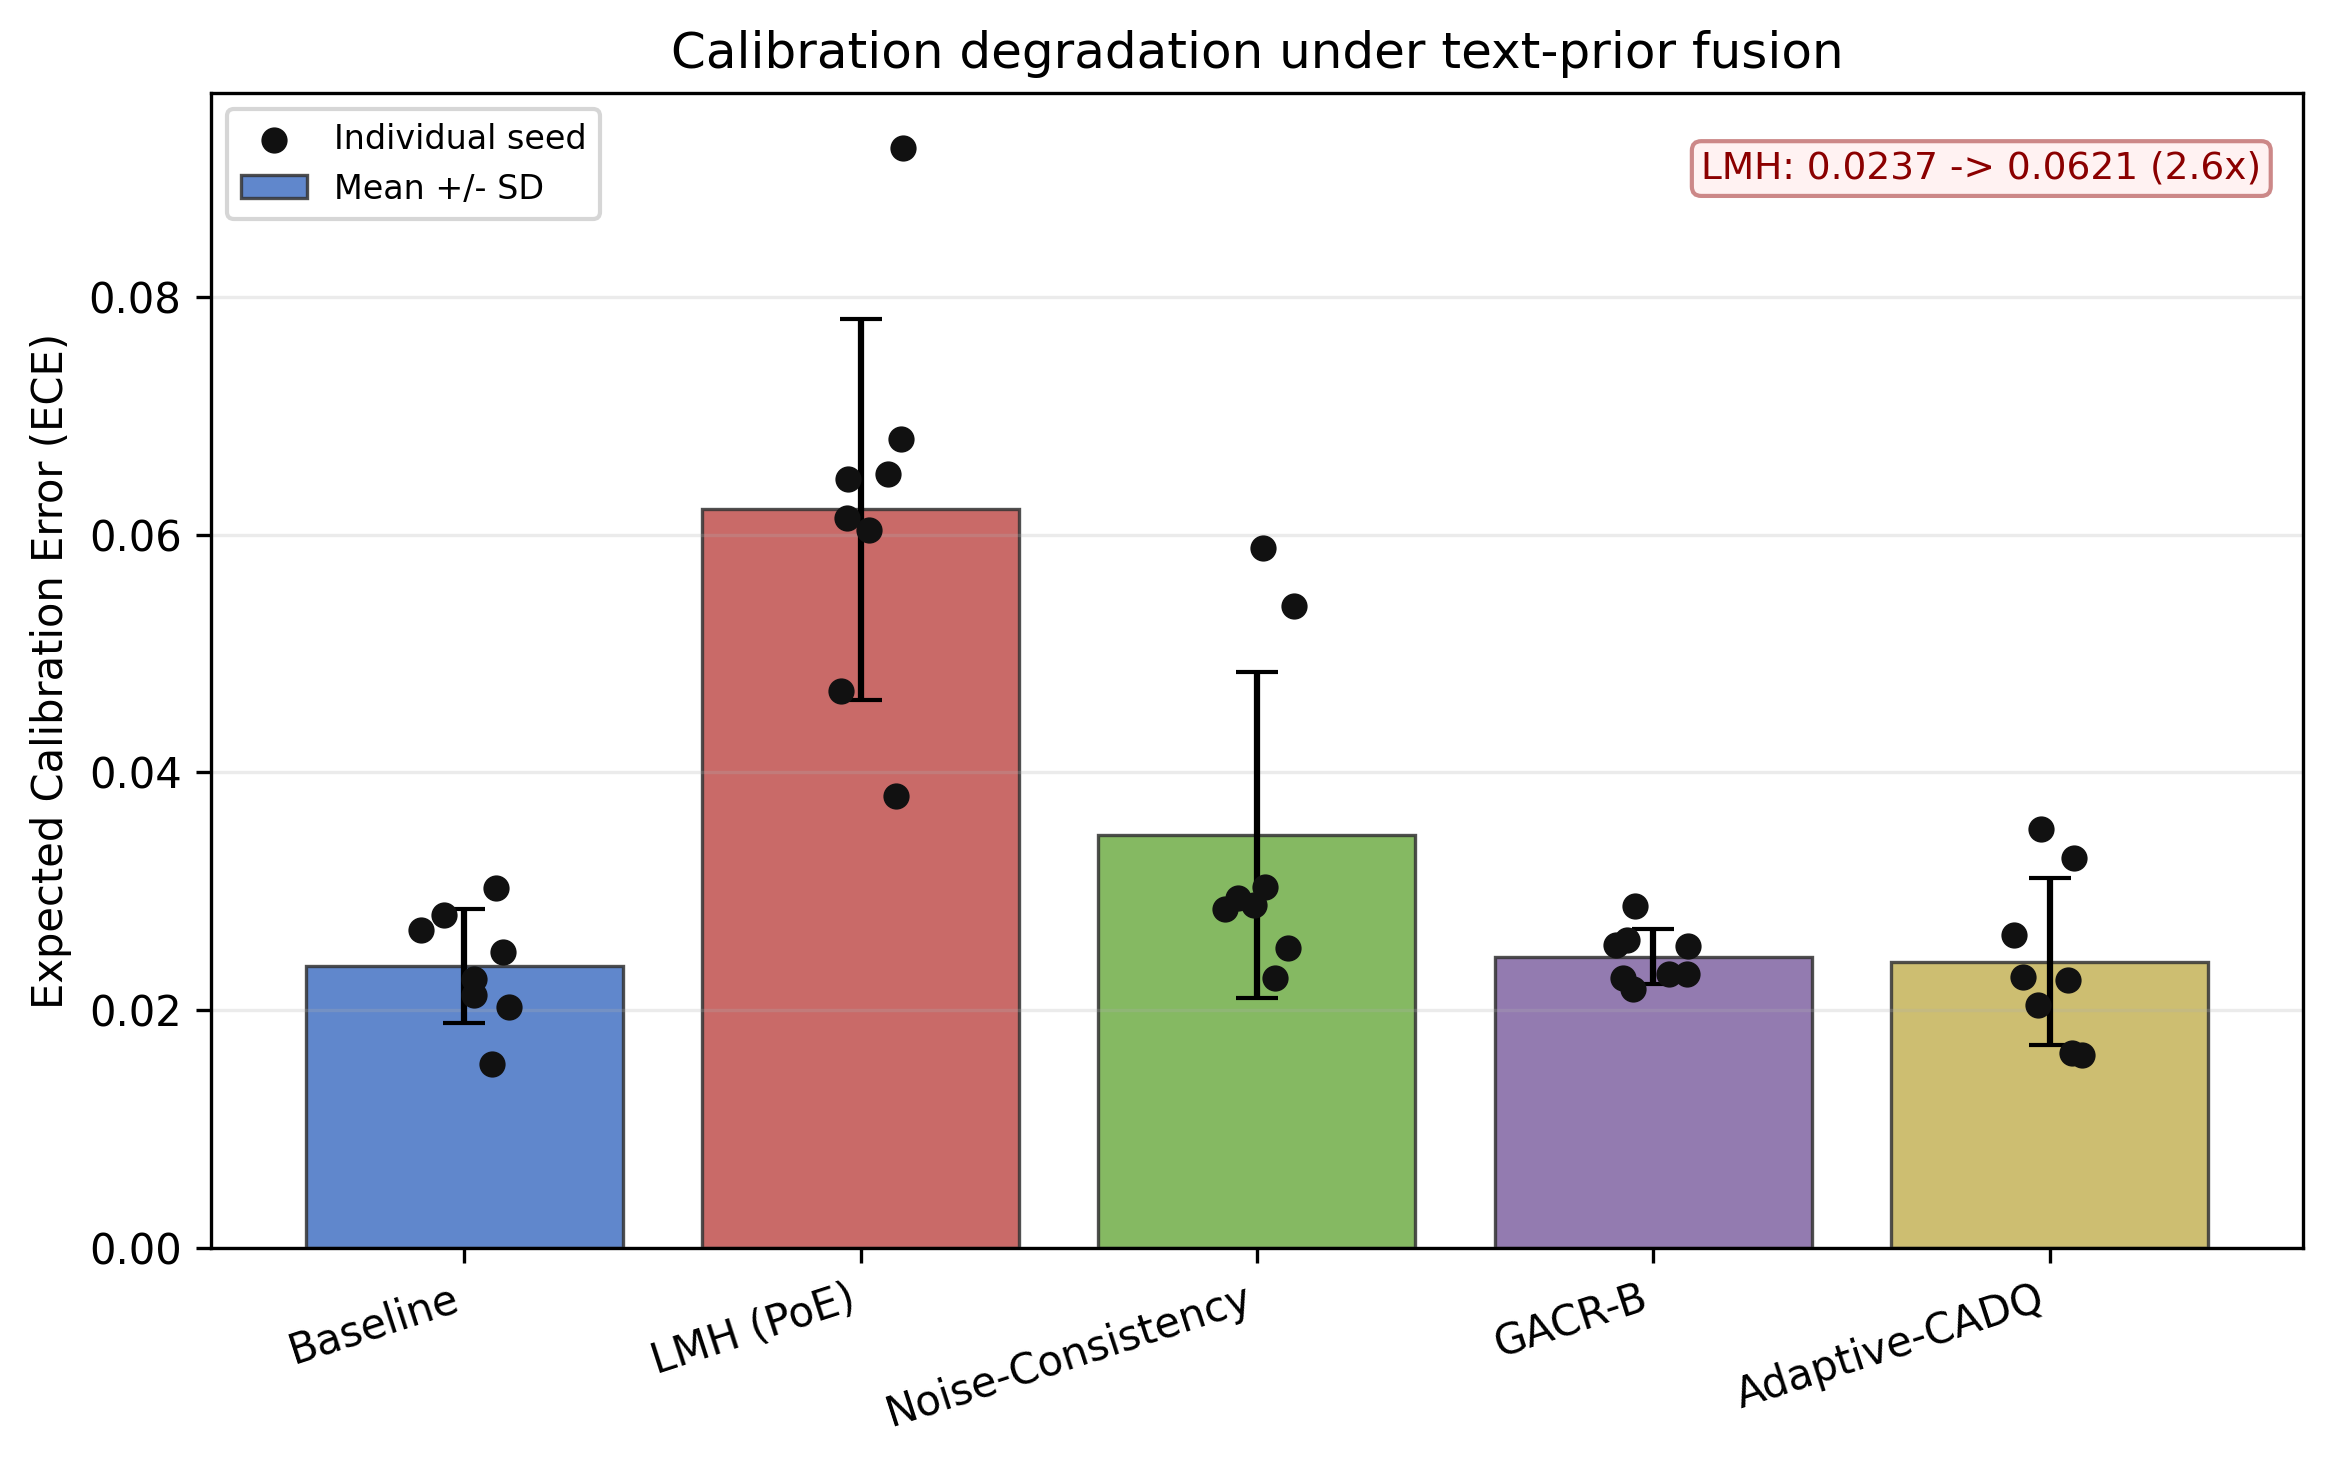
\includegraphics[width=\linewidth]{ece_seed_dots.png}\par
\textbf{(b)}
\end{minipage}
\caption{Baseline reliability and seed-level expected calibration error.}
\label{fig:calibration}
\end{figure*}

\subsection{Report-preserving controls and ICM}\label{sec:icm}

The retained image-only control achieved Macro-F1 0.4611, accuracy 0.5670,
Macro-AUROC 0.6728, ECE 0.0993, and Brier score 0.6142. The text-only control
achieved 0.8555, 0.9077, 0.9820, 0.0203, and 0.1289, respectively. The
Gray-Square control achieved Macro-F1 0.9381, accuracy 0.9604, Macro-AUROC
0.9960, ECE 0.0369, and Brier score 0.0589. Its Macro-F1 was only 0.0016 below
the baseline eight-seed mean. Because these were single retained runs and the
image-only pipeline did not guarantee restoration of the best validation
checkpoint, they support an audit of
the archived system but not a definitive ranking of modality capacity.

Baseline ICM was $0.0016\pm0.0065$ with median 0.0014 and bootstrap 95\%
confidence interval $[-0.0026,0.0061]$ (Table~\ref{tab:icm}). The signed-rank
test did not reject zero ($p=0.4219$), while TOST supported equivalence inside
the operational interval ($p=0.0040$). LMH had ICM $0.0056\pm0.0098$ and did
not meet the equivalence criterion. The noise-sensitivity (anti-consistency)
condition had a negative mean ICM ($-0.0039\pm0.0081$), whereas exploratory
GACR-B and Adaptive-CADQ had small
positive values. None showed a robust positive contribution relative to the
Gray-Square reference.

The baseline estimate is central because its confidence interval straddles
zero while remaining within the predeclared operational bounds. The Wilcoxon
result alone would only show that the retained seeds do not establish a
difference from zero. The TOST result supplies the additional, bounded claim
that the effect is compatible with the chosen near-zero interval. This is an
operational statement about Macro-F1 in this cohort, not proof of exact equality
and not a clinical non-inferiority margin.

The confidence intervals in Table~\ref{tab:icm} are percentile bootstrap
intervals from 2,000 seed resamples. The Wilcoxon column tests ICM against zero,
whereas TOST asks whether it lies inside the operational interval. These tests
answer different questions and are therefore reported together.

\begin{table*}[t]
\centering
\caption{Seed-level Image Contribution Metric statistics.}
\label{tab:icm}
\scriptsize
\resizebox{0.94\textwidth}{!}{%
\begin{tabular}{lrrrrrrr}
\toprule
Condition & Mean & SD & Median & 95\% CI & Wilcoxon $p$ & TOST $p$ & Cohen's $d$ \\
\midrule
Baseline & 0.0016 & 0.0065 & 0.0014 & $[-0.0026,0.0061]$ & 0.4219 & 0.0040 & 0.247 \\
LMH (PoE) & 0.0056 & 0.0098 & 0.0066 & $[-0.0011,0.0118]$ & 0.1953 & 0.1223 & 0.566 \\
Noise-sensitivity (anti-consistency) & -0.0039 & 0.0081 & -0.0009 & $[-0.0097,0.0009]$ & 0.3828 & 0.0345 & -0.476 \\
Exploratory GACR-B & 0.0038 & 0.0062 & 0.0030 & $[-0.0002,0.0081]$ & 0.1953 & 0.0122 & 0.607 \\
Adaptive-CADQ & 0.0007 & 0.0077 & 0.0002 & $[-0.0043,0.0057]$ & 0.8438 & 0.0054 & 0.089 \\
\bottomrule
\end{tabular}}
\end{table*}

The seed pairing, equivalence interval, and retained gate values are shown in
Fig.~\ref{fig:icm-gates}. The Gray-Square value was reused for all eight ICM
calculations; its run-to-run uncertainty is therefore absent from the displayed
intervals. The equivalence result should be interpreted as a property of the
retained comparator, not an estimate from two independently replicated arms.

\begin{figure*}[t]
\centering
\begin{minipage}[t]{0.32\textwidth}
\centering
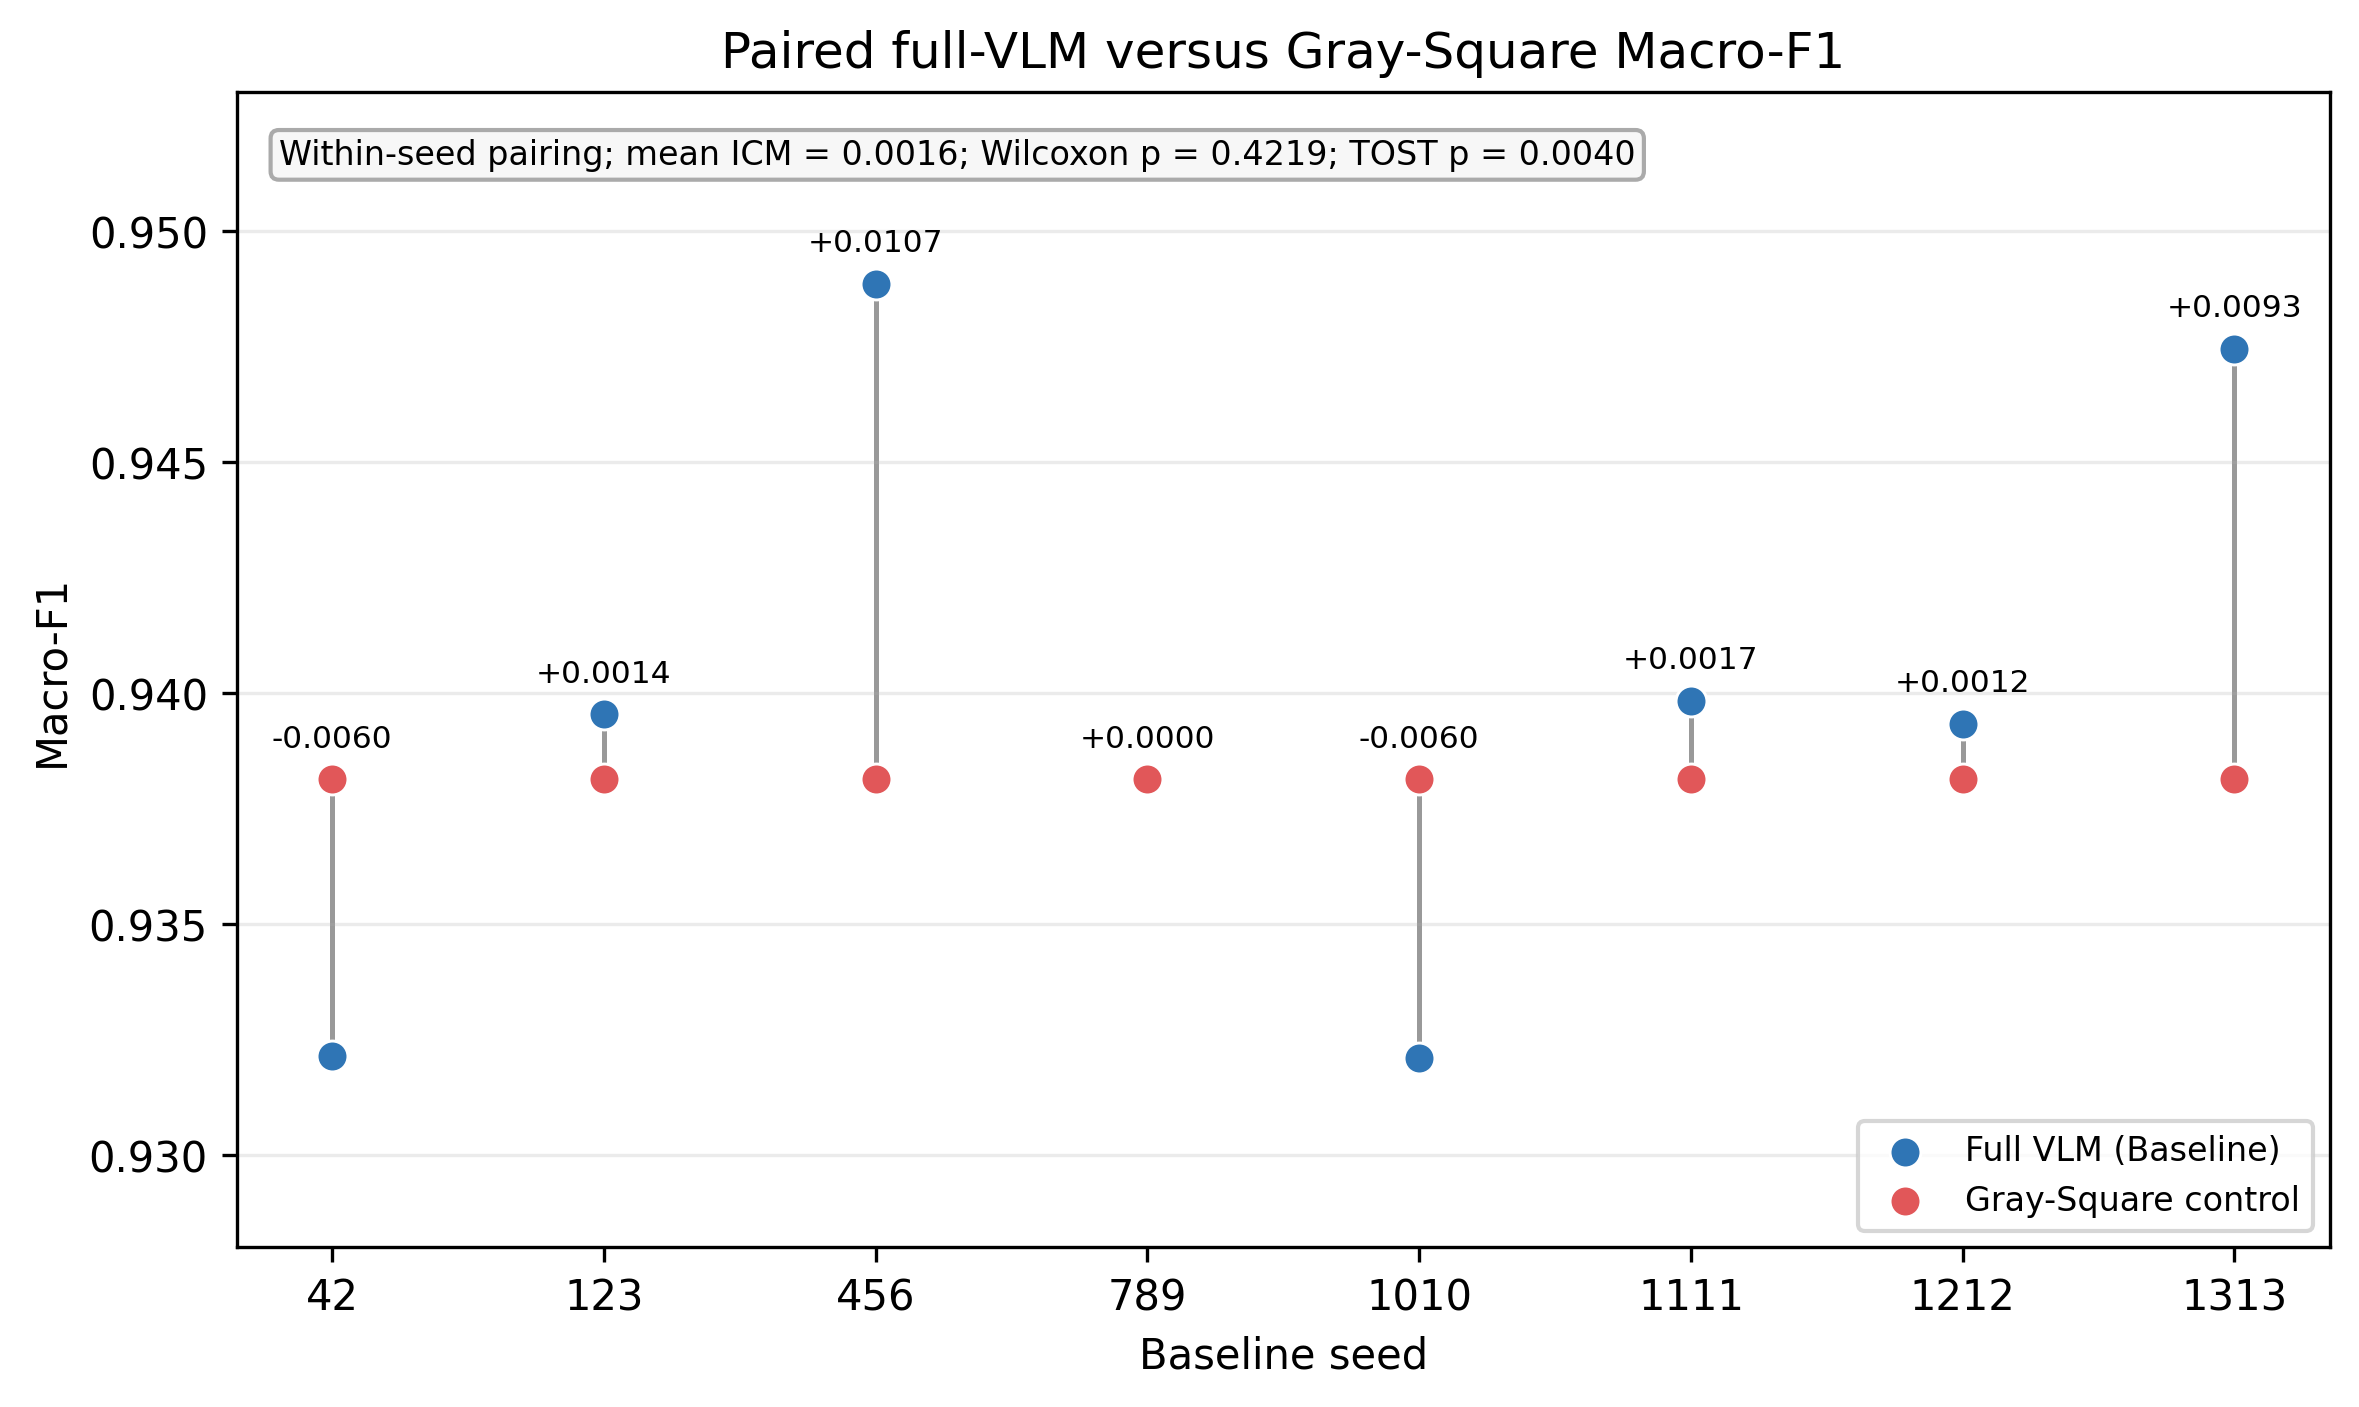
\includegraphics[width=0.98\linewidth]{paired_vlm_gray_square.png}\par
\textbf{(a)}
\end{minipage}\hfill
\begin{minipage}[t]{0.32\textwidth}
\centering
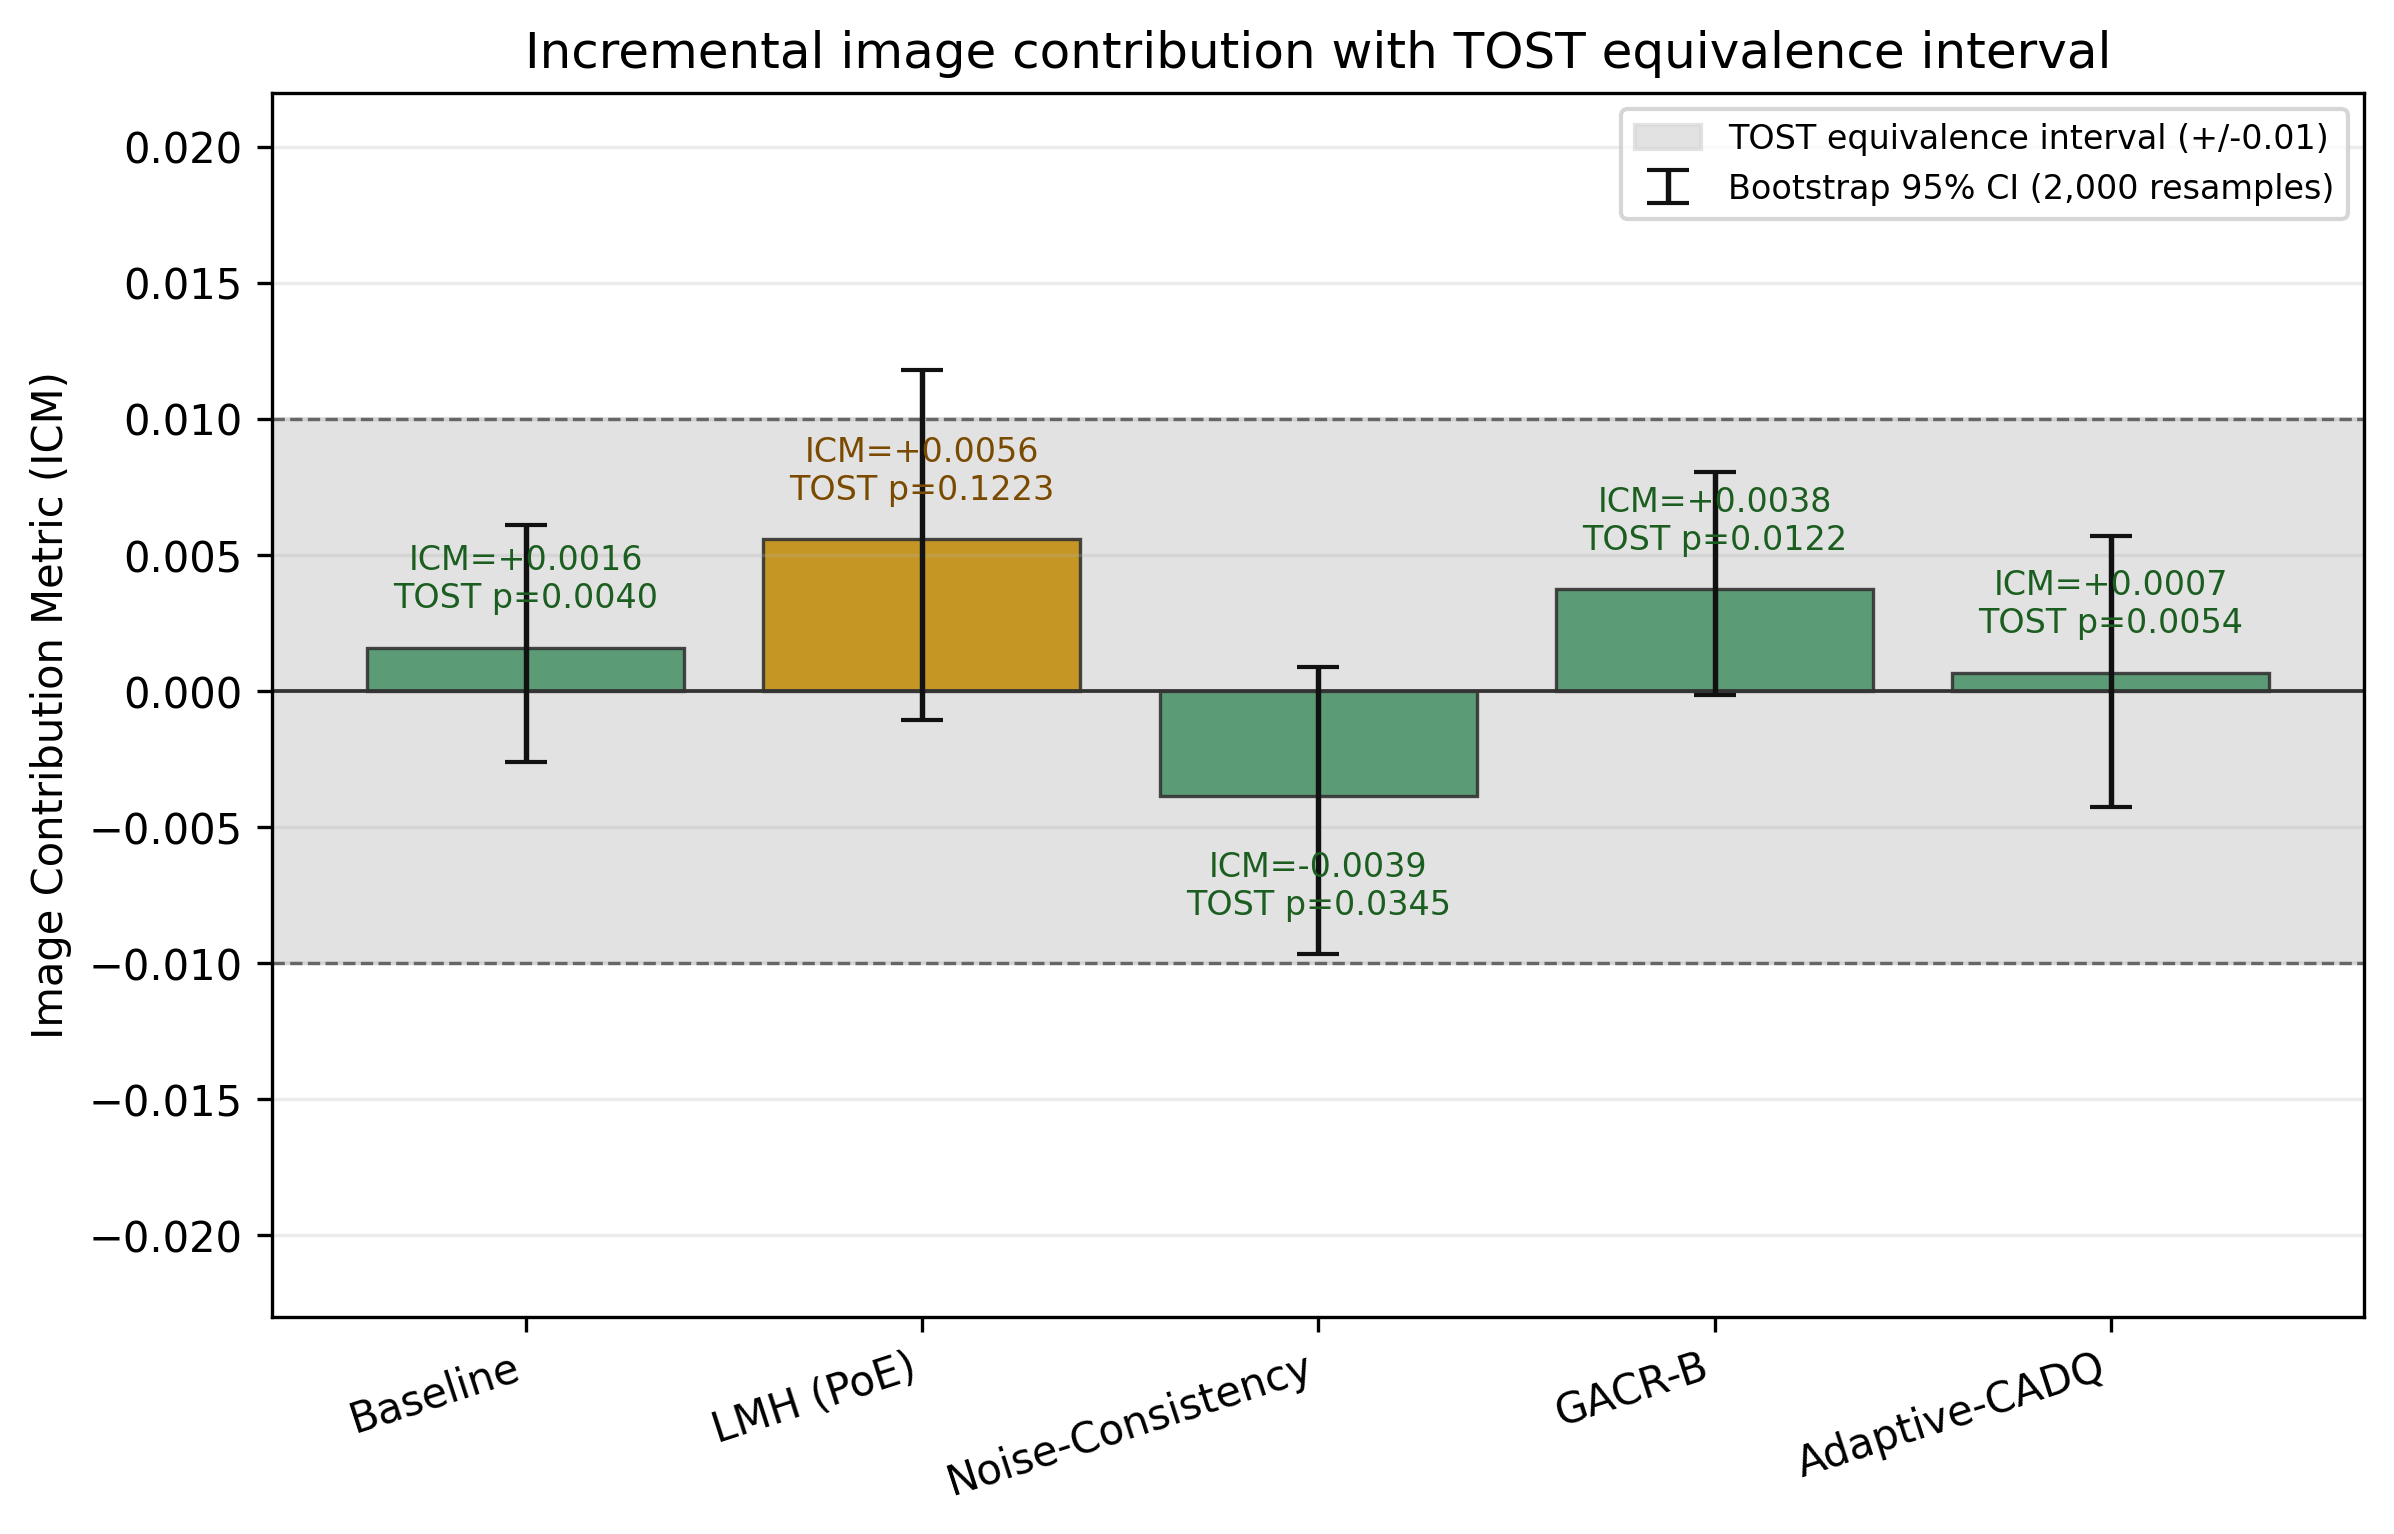
\includegraphics[width=0.98\linewidth]{icm_tost_master.png}\par
\textbf{(b)}
\end{minipage}\hfill
\begin{minipage}[t]{0.32\textwidth}
\centering
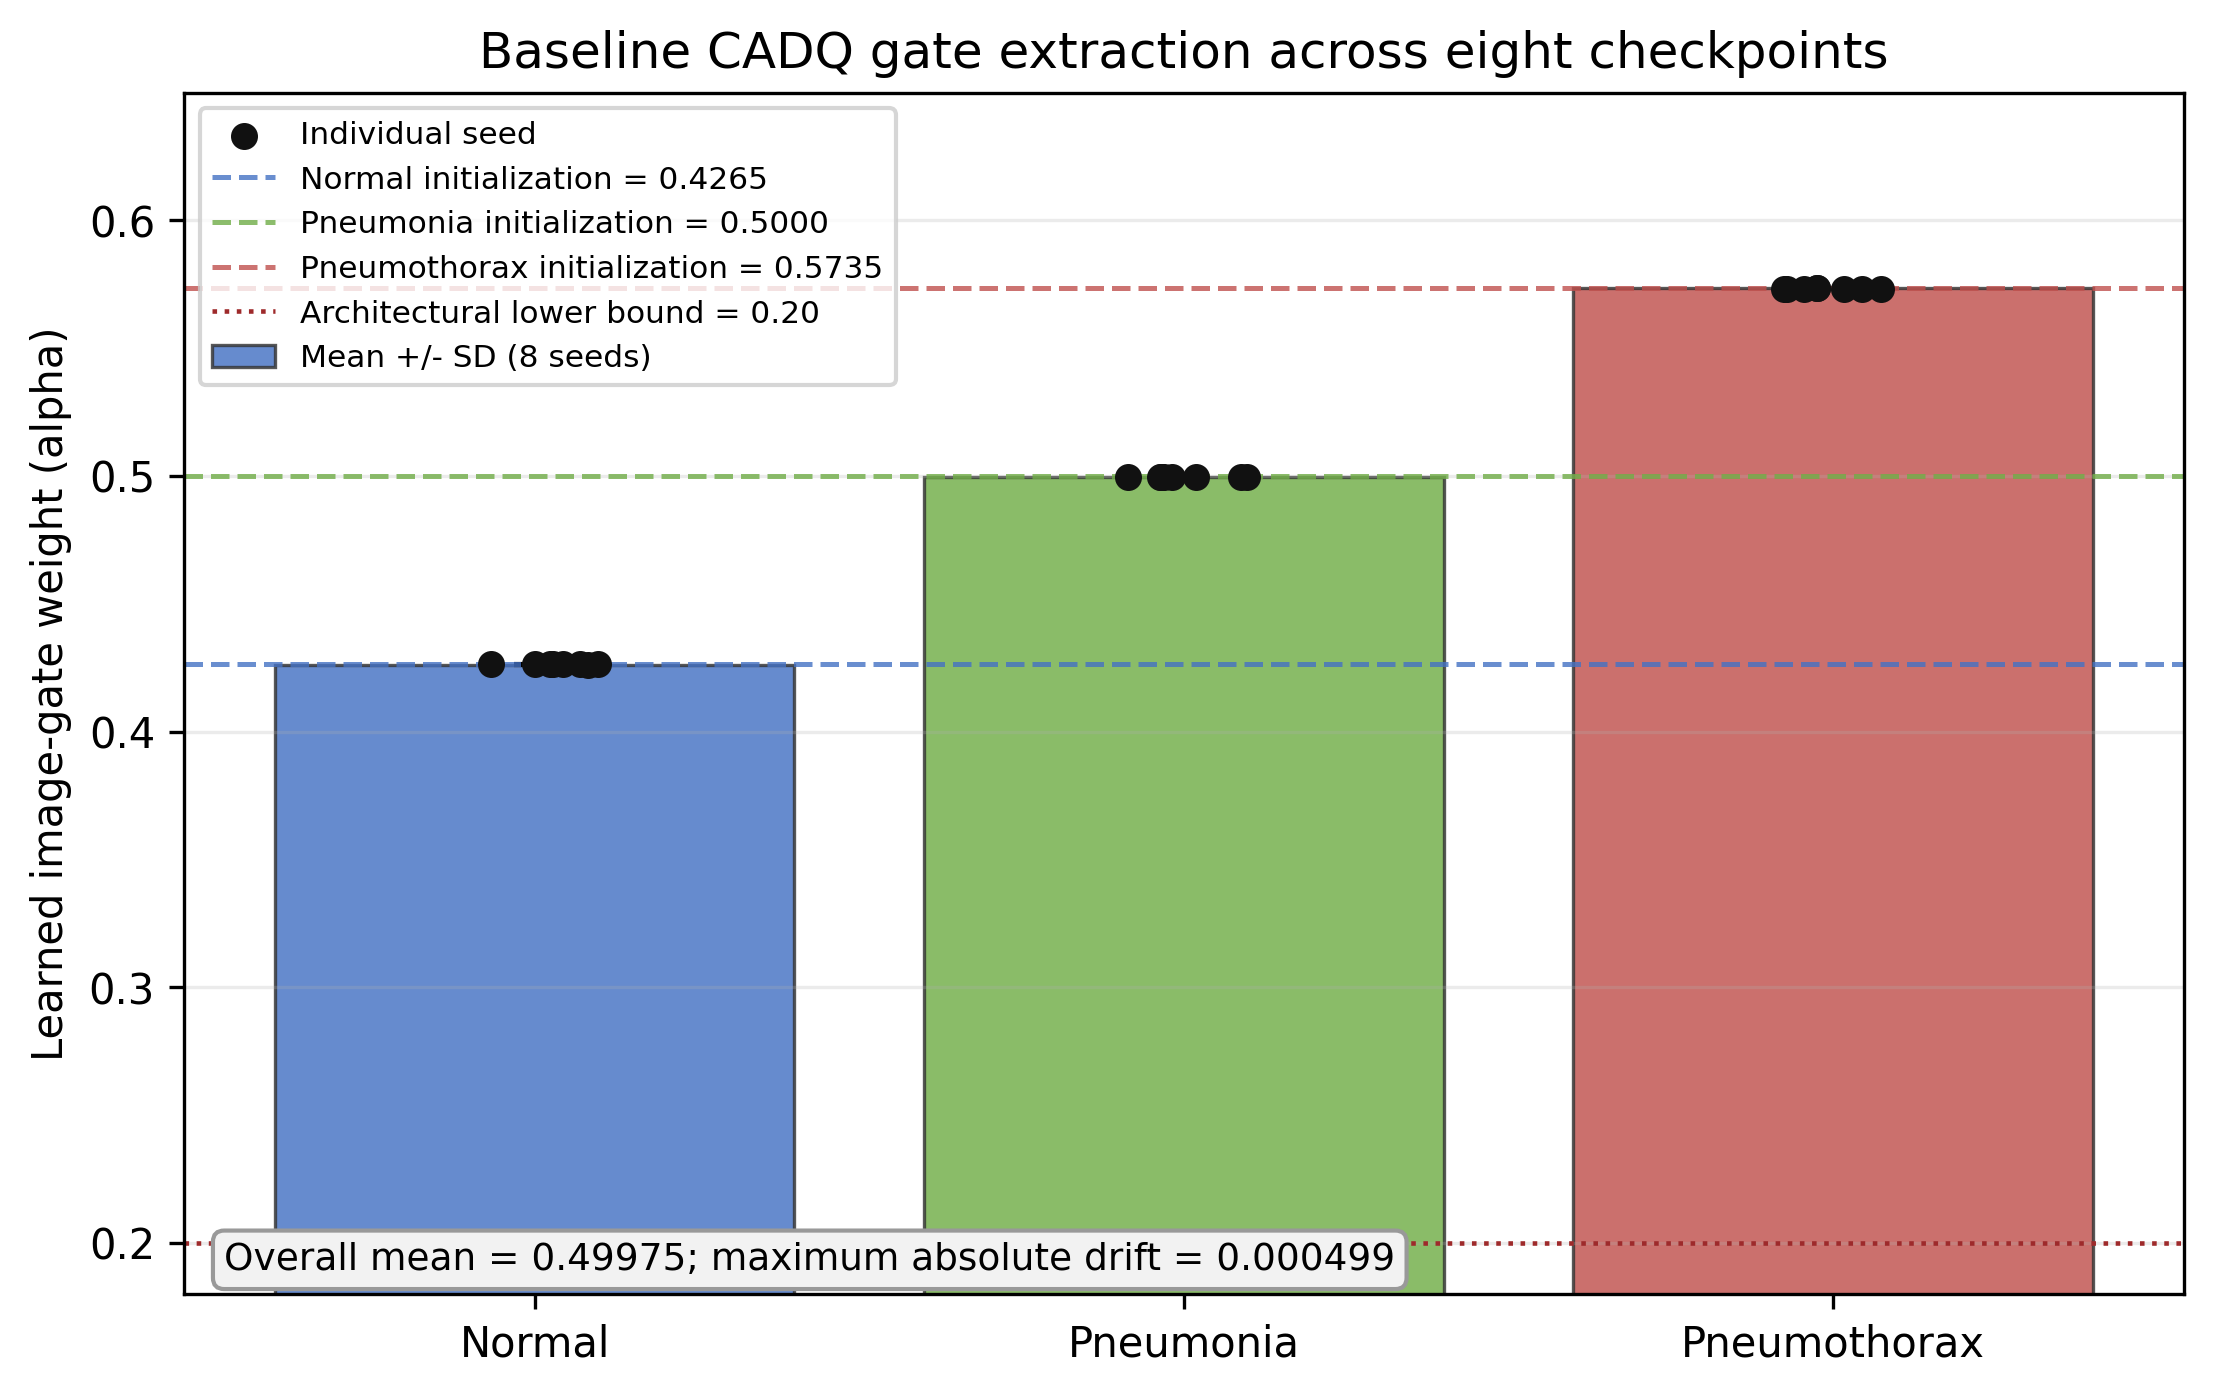
\includegraphics[width=0.98\linewidth]{gate_stagnation_with_dots.png}\par
\textbf{(c)}
\end{minipage}
\caption{Paired image ablation, ICM equivalence, and retained baseline gates.}
\label{fig:icm-gates}
\end{figure*}

\subsection{Gate behaviour and qualitative inspection}\label{sec:gates}

The retained baseline gate means were 0.42624 for Normal, 0.49963 for
Pneumonia, and 0.57336 for Pneumothorax. The overall mean was 0.49975 compared
with an initialization mean of 0.50000, and the largest per-seed class-wise
deviation from the equation-derived initialization was 0.000499. The gate did
not collapse toward its lower bound of 0.20, nor did the retained values show a
meaningful shift toward greater image reliance. We call this descriptive pattern
\emph{gate stagnation}; it is evidence that this parameter changed little, not
proof that its gradient was exactly zero or that the image branch was
disconnected. Per-seed values appear in Supplementary Table~\ref{tab:s-gates}.

The class-specific means track the deliberately different initial values rather
than converging on a common boundary. This pattern explains why a nominal gate
near 0.5 cannot be read as evidence that half of the decision came from the
image. The gate equation allocates weight between logits, but the represented
features can be redundant and the parameter can remain almost unchanged. The
behavioural Gray-Square comparison is therefore the stronger source of evidence
about incremental image information.

The three retained Grad-CAM examples showed diffuse activation in Baseline seed
42 (Supplementary Fig.~\ref{fig:s-gradcam}). They were not compared with
localization annotations, deletion curves, or clinician assessment. They
therefore provide only a qualitative sanity check and cannot establish visual
grounding or its absence.

\subsection{Synthesis across evidence sources}\label{sec:result-synthesis}

The result set is internally consistent when each analysis is assigned its
proper scope. Baseline discrimination is high, but the report-preserving
control retains nearly the same Macro-F1. The baseline ICM confidence interval
crosses zero and fits inside the operational equivalence range under TOST. The
static gate remains close to initialization, and the qualitative saliency
examples do not supply independent localization evidence. None of these
observations alone proves the absence of visual information; together they
show that the evaluated Macro-F1 provides little evidence of incremental image
use in the retained setting.

The intervention results also explain why the cross-variant table should not be
read as a simple ranking. LMH has the largest mean Macro-F1, yet its AUROC and
calibration are worse than baseline. Exploratory GACR-B has the largest small
positive ICM among the tested variants, but the adjusted Macro-F1 comparison
does not establish improvement. Adaptive-CADQ retains baseline-like
discrimination and calibration without increasing ICM. The
noise-sensitivity (anti-consistency) condition changes the objective but does
not produce a positive contribution estimate. No condition satisfies the
combined requirement of improved incremental image contribution without an
offsetting loss in the reported evidence.

Class-specific results place the aggregate finding in context. Pneumothorax has
the smallest test count and the widest variation, so small numerical changes in
its F1 require more caution than equally sized changes in the Normal class.
Seed-42 sensitivity intervals overlap across conditions, and the descriptive
confusion matrices do not reveal a new, stable rare-class advantage. This does
not eliminate the possibility of a clinically important subgroup effect; it
shows that such an effect is not established by the retained cohort and
outputs.

Finally, the evidence distinguishes reproducibility from breadth. Forty
condition-seed records support paired seed-level summaries for the five fusion
conditions. The controls, DeLong analysis, and McNemar analysis have narrower
retained coverage. Their value lies in answering specific audit questions, not
in implying that every component has the same replication depth. This coverage
is repeated in the supplementary provenance manifest so that readers can trace
each numerical claim to the available output type.

% Keep the complete quantitative Results display set ahead of interpretation.
\FloatBarrier
\section{Discussion}\label{sec:discussion}

This section interprets the findings at three levels. It first examines what
the Gray-Square result establishes about the evaluated construct, then relates
the fusion and calibration results to prior modality-bias work, and finally
sets out the conditions required for broader biomedical or clinical use. The
discussion keeps behavioural evidence separate from possible optimization
mechanisms so that a descriptive audit is not presented as a causal account of
training dynamics.

\subsection{Principal findings and interpretation}\label{sec:principal}

The central result is a mismatch between high predictive performance and
incremental image evidence. Baseline Macro-F1 approached 0.94, yet a constant
gray image paired with the same report retained Macro-F1 0.9381. Baseline ICM
was close to zero, its signed-rank test was non-significant, and TOST supported
equivalence within the project-defined interval. None of the four alternative
fusion or text-debiasing conditions produced a robust ICM increase. The LMH
text-prior intervention had the highest mean Macro-F1 but lower AUROC and much
worse calibration. The retained baseline gates stayed close to initialization.
Together, these findings show that aggregate performance, a non-collapsed gate,
and visually plausible activation maps can coexist with negligible performance
change after image replacement.

This combination is more informative than any component alone. High baseline
performance shows that the task is predictable under the available inputs. The
Gray-Square contrast asks whether image content adds to that prediction. TOST
places the observed difference within an operational interval, and gate
extraction checks whether the fusion parameter moved during training. The four
steps narrow the interpretation from ``the model performs well'' to ``the model
performs well even when image content is removed under this retained
report-linked setting.''

\subsection{Construct validity and modality inertia}\label{sec:construct}

The most direct explanation is construct overlap. MIMIC-CXR pairs each image
with a report, CheXpert uses report language to generate the target, and the
model receives the report's \texttt{findings} field
\cite{johnson2019mimiccxr,irvin2019chexpert}. The Gray-Square control preserves
this high-information route. It does not show that the CheXpert labels are
clinically inaccurate, that every prediction copied a particular phrase, or that
radiographs lack diagnostic value. It shows that the evaluated endpoint does
not isolate independent image-based recognition. The claim supported by the
data is therefore narrow: under this report-linked setup and archived
implementation, the measured incremental image contribution was negligible.

The distinction is one of construct validity. If the intended construct is
independent visual recognition, a target generated from the same report given
to the model does not isolate it. If the intended construct is report-linked
classification, the task remains internally coherent, but the meaning of the
score changes. The same numerical result can therefore be appropriate for one
use and misleading for another. A clear target-provenance statement is needed
before performance is compared with image-only or independently labelled
systems.

We use \emph{modality inertia} to describe the combined observation that the
output changes little under report-preserving image replacement while the
static gate remains near its starting value. This is a useful diagnostic label,
but the current experiment does not identify a unique mechanism. Redundant
features, optimization dynamics, precision, normalization mismatch, or weak
image gradients could each contribute. The gate result should not be promoted
from a parameter-stability observation to proof of causal gradient starvation
without gradient traces or controlled retraining.

The term also avoids a false choice between gate collapse and successful
fusion. A gate can stay comfortably inside its bounds while the output remains
insensitive to the image. That outcome is possible when the two pathways encode
overlapping evidence or when one pathway already predicts the report-derived
target. Gate values should therefore be interpreted together with ablations,
not converted directly into percentages of causal contribution.

\subsection{Interpretation of the tested conditions}\label{sec:variants}

The debiasing results clarify why endpoint design matters. Product-of-experts
methods are intended to suppress an easy language prior. Here, however, report
language helped generate the target. Down-weighting this pathway can degrade
AUROC or calibration without creating new image information, as observed for
LMH. The noise-sensitivity (anti-consistency) condition cannot support its
intended conventional-consistency interpretation because its archived
negative-KL formulation rewards divergence. Adaptive-CADQ changed the gate form
but not the endpoint. Exploratory GACR-B, following the grounding-aware
proposal of Sadanandan and Behzadan
\cite{sadanandan2026consistentdangerous}, achieved a small ICM but not a robust
Macro-F1 improvement. The experiment did not measure whether its $\lambda=0.3$
penalty generated insufficient gradient; that mechanism requires a dedicated
ablation and is not inferred from the null performance result.

These findings do not show that debiasing is generally ineffective. They show
that each intervention is evaluated against the information structure of its
target. Product-of-experts methods can be useful when a language prior is a
spurious correlate; noise-based objectives can be useful when their loss
encourages stable predictions; adaptive gates can respond when modality
uncertainty is informative; and grounding-aware penalties can matter when the
reference standard rewards the intended evidence. In this experiment, none of
those changes established a reliable gain over the report-preserving control.
The relevant conclusion concerns the fit between method and benchmark, not a
universal ranking of algorithms.

The corrected McNemar interpretation is also important. Exploratory GACR-B and
Adaptive-CADQ had $p=1.000$, but both had non-zero discordant predictions. The
off-diagonal counts were nearly balanced, so McNemar detected no directional
change in error rates. This supports a conclusion of similar aggregate paired
behaviour, not byte-identical decision boundaries. Reporting the contingency
counts prevents a non-significant symmetry test from being mistaken for an
identity test.

Calibration provides a second reason to avoid ranking conditions from Macro-F1
alone. LMH reached the highest unadjusted mean Macro-F1 but increased ECE by a
factor of 2.6 and increased Brier score. A system can preserve its predicted
class while changing probability quality enough to affect threshold-based use.
For biomedical evaluation, a debiasing objective should therefore be judged by
discrimination, calibration, and modality contribution together.

\subsection{Implications for biomedical informatics}\label{sec:implications}

The practical implication is a change in evaluation sequence. Target
provenance should be mapped before a multimodal architecture is trained.
Modality controls should then be matched to the intended claim, and only after
that should aggregate performance be interpreted. This order helps separate a
useful report-conditioned predictor from a claim of independent visual
reasoning.

Multimodal evaluation should make modality contribution explicit. A minimum
audit should document how targets were produced, whether any input shares that
source, what happens when each modality is replaced or permuted, whether
controls are matched across seeds, and how calibration changes. The ablation
must preserve all other inputs and the evaluation cohort. Where the scientific
claim is that an image contributes, an independent or image-derived reference
standard is preferable to a target extracted from the accompanying report.
Counterfactual text tests, temporally separated note fields, and cross-patient
report swaps can further reveal which source carries the prediction.

Prior studies support this sequence from different directions. Image-text
learning establishes the value of report supervision
\cite{zhang2022convirt,huang2021gloria,boecking2022textsemantics}; context and
image-removal studies show that apparent multimodal performance can persist
without the intended visual evidence
\cite{wang2026clinicalcontext,lotfinia2026needimage}. The audit taxonomy of
Sadanandan and Behzadan provides a broader framework for interpreting that
behaviour \cite{sadanandan2026consistentdangerous}. The present study adds a
seed-level relative measure, an operational equivalence test, and retained-gate
inspection. These forms of evidence are complementary rather than
interchangeable.

ICM is one compact summary of such an intervention. Its advantages are an
interpretable direction and a model-relative scale, but it inherits every
limitation of the chosen performance metric and comparator. Macro-F1 may hide
class-specific harm; a single Gray-Square run understates control uncertainty;
and the $[-0.01,0.01]$ interval has not been clinically validated. ICM should
therefore be reported with absolute performance, per-class outcomes,
calibration, confidence intervals, and a description of the control. Validation
on independent-label tasks is needed before comparing ICM across datasets.

Gate and saliency analyses should remain secondary. A gate is shaped by
parameterization and can be unidentifiable when modality signals are redundant.
The one-key attention block used here cannot align words to image regions, and
three Grad-CAM examples lack quantitative localization evidence. A stronger
future design would use token- and region-level interactions, paired modality
interventions, gradient and gate trajectories, concept localization, and
reader-validated explanations. Even then, behavioural change under input
intervention remains the more direct evidence of contribution.

Reporting should also distinguish primary and supporting evidence. A compact
minimum set would include the full-condition metric, a matched ablation, the
absolute and relative difference, uncertainty over independent training runs,
class-specific outcomes, and calibration. Architecture parameters and
explanations can be added when their scope is explicit. CLAIM and TRIPOD+AI
provide useful structures for data, modelling, and validation, while a
modality-provenance table and intervention result make the specific information
flow easier to audit \cite{mongan2024claim,collins2024tripodai}.

For regulatory-facing evidence, the central lesson is traceability rather than
a proposed mandatory threshold. Good machine-learning-practice and real-world-
evidence principles emphasize representative evaluation, transparent data
provenance, uncertainty, and evidence aligned with intended use
\cite{fda2025gmlp,fda2025rwe}. A multimodal device dossier should therefore
state whether labels and inputs share provenance and include matched ablations
when modality use is part of the intended claim. ICM and gate inspection can
support that evidence package, but neither substitutes for external validation,
clinical utility, subgroup performance, or human-factors assessment.

\subsection{Requirements for broader validation}\label{sec:validation-design}

A broader study should first break the target-input dependence. The preferred
reference would be an image-derived label established independently of the
report text given to the model, with adjudication rules and uncertainty handling
specified before evaluation. If report-conditioned prediction is the intended
task, that use should be stated directly and compared with a text-only system.
The key requirement is alignment between the claimed capability and the source
of the reference standard.

Control replication is the next priority. Full VLM, Gray-Square, text-only, and
image-only conditions should be trained under the same seed schedule and
checkpoint rule. Image replacement can be complemented by image permutation,
cross-patient replacement, region masking, and report perturbation. Those
interventions should be selected according to the question: replacement tests
whether image content matters at all, permutation tests whether image-report
pairing matters, and localized masking tests whether specific regions affect
the output. A single control cannot answer all three.

The statistical design should specify the replication unit and minimum relevant
effect before model fitting. When several seeds are paired to the same control,
both sides of the comparison should carry replicated uncertainty. Subject-level
ROC and error tests should use matched predictions from the same seed or an
explicit hierarchical model rather than concatenating repeated patients.
Equivalence margins should be justified for the chosen metric and intended use;
the operational $[-0.01,0.01]$ interval in this study is a transparent project
definition, not a transferable clinical standard.

Evaluation should extend beyond one aggregate score. Class-specific sensitivity
and precision are needed when prevalence and clinical consequences differ.
Calibration should be assessed before and after any probability adjustment,
with thresholds selected on validation data. Subgroup analyses should be
planned for demographic, acquisition, and institutional factors that are
available and ethically appropriate. External evaluation should preserve the
target definition or explicitly explain how a different label process changes
the estimand.

Mechanistic claims require their own measurements. To test whether weak gradient
signal explains gate stagnation, an experiment would need gate and gradient
trajectories, controlled initialization, full-precision checks, and training
under an independently labelled endpoint. To assess spatial grounding,
qualitative heatmaps should be supplemented by expert localization, deletion or
insertion tests, and reader assessment. These measurements would connect
internal model behaviour to the intervention result without treating a single
visualization as causal evidence.

Finally, the evidence chain should be recoverable. A release should map every
condition to the source notebook, dataset and split hashes, software
environment, checkpoint rule, seed, probability array, prediction file, and
figure-generation command. This form of provenance is useful even when raw
clinical data cannot be redistributed. It allows a reviewer to distinguish a
reproducible numerical result from an interpretation that depends on an
unstated processing choice.

\subsection{Study boundaries}\label{sec:limitations}

This audit has substantial limitations. It used 2,953 studies from one
database, one labeler, three classes, and only 47 Pneumothorax test studies. The
uncertain-to-negative mapping, class caps, prevalence, and inherited split may
affect the results. No external cohort, radiologist-adjudicated reference,
prospective workflow, reader study, subgroup analysis, decision-curve analysis,
or outcome evaluation was available. Generalization to other reports,
institutions, devices, and label processes is unknown.

Implementation limitations constrain causal interpretation. Residual
non-uniform effects of the $[-1,1]$ mapping cannot be fully excluded; it is
treated as a shared preprocessing constraint across all conditions
\cite{cohen2022torchxrayvision}. The noise-sensitivity (anti-consistency) condition
used a negative-KL formulation that rewards divergence. The attention block
used one token per modality. Image-only checkpoint restoration did not
guarantee the best validation checkpoint, so that control is descriptive.
The affected conditions are interpreted as probes of the archived system's
behaviour under a report-linked endpoint. ICM and condition contrasts are the
primary evidence within this setting; although shared preprocessing makes
condition-specific effects unlikely, residual non-uniform effects cannot be
fully excluded.

Control and statistical asymmetries also matter. The same single Gray-Square
run was reused to construct eight ICM values, so comparator uncertainty was not
propagated. Eight seeds provide a small replication sample. DeLong and McNemar
results were computed only from the retained seed-42 arrays, whereas
seed-aggregated curves are descriptive. Adaptive-CADQ's eight-seed extension and
exploratory GACR-B were post hoc. No a priori sample-size calculation established power for
a clinically meaningful ICM. Future studies should train every control at every
seed, preregister the equivalence margin and estimand, and use a larger
independent-label cohort.

The ICM formulation has additional measurement boundaries. Because it is
normalized by the full-model Macro-F1, it can become unstable for poorly
performing models and should always be reported beside the absolute difference.
The constant gray tensor removes anatomical information but can also create an
input distribution that differs from natural radiographs. A cross-patient image
swap or matched permutation control would test pairing dependence with more
natural image statistics. The current study did not retain such a replicated
control, so its conclusion is specific to the Gray-Square intervention.

The supporting analyses are narrower than the primary endpoint. Gate values
were available for baseline checkpoints but not as full trajectories for every
condition. The small numerical drift is compatible with stagnation, yet the
retained precision limits fine-grained interpretation. Grad-CAM was available
for three baseline seed-42 examples without expert spatial annotations. These
examples can reveal obvious qualitative behaviour, but they do not measure
localization accuracy or the causal effect of a highlighted region.

Finally, the result archive was assembled from multiple notebook outputs. The
merge retained first-seen duplicates without a documented source-priority rule
or content hashes, and some probabilities had to be recovered from a companion
pickle. A confirmatory release should include a locked environment, dataset and
split hashes, notebook and checkpoint hashes, deterministic merge rules, full
probability arrays, and a machine-readable provenance manifest. The present
manifest is descriptive and identifies rather than resolves these issues.

\section{Conclusion}\label{sec:conclusion}

In this MIMIC-CXR-derived task, replacing the radiograph with a constant image
preserved nearly all baseline Macro-F1. Baseline ICM was near zero and equivalent
within the operational interval, the tested interventions did not demonstrate a
robust increase in incremental image contribution, and retained static gates
remained near initialization. These findings expose a benchmark-validity risk
created when labels and text inputs share report provenance. They do not show
that radiographs or medical VLMs are generally uninformative. Independent
labels, implementation validation, matched multi-seed controls, provenance
locking, and external validation are required. ICM is best used as one component
of a broader modality-reliance audit.

\section*{Ethics approval and consent to participate}
MIMIC-CXR is de-identified and was accessed through official PhysioNet
credentialing under its Data Use Agreement. No participants were recruited, no
direct identifiers were accessed, and consent was not applicable. The source
resource was released under the originating institutional review-board
approvals; this secondary computational analysis introduced no intervention or
participant contact.

\section*{Data availability}
Raw MIMIC-CXR images and reports remain under PhysioNet access controls and are
not redistributed. Non-identifying summaries, code, manuscript source, and
figure-generation materials are available at
\url{https://github.com/i-mTanvir/MediVision}. Cohort identifiers can be shared
only in a manner consistent with the PhysioNet Data Use Agreement.

\section*{Code availability}
The analysis notebooks, LaTeX source, figure scripts, and environment records
are available at \url{https://github.com/i-mTanvir/MediVision}. A permanent
archival DOI will be added if a versioned release is deposited. Credentials,
raw reports, and restricted identifiers are excluded.

\section*{Funding}
This research received no specific grant from public, commercial, or
not-for-profit funding bodies and was self-funded by the authors. No external
sponsor influenced the design, analysis, interpretation, writing, or decision
to submit.

\section*{Declaration of competing interest}
The authors declare no known competing financial interests or personal
relationships that could have influenced this work.

\section*{Author contributions}
Nafis Al Rahman and Tanvir Mahmud contributed equally to conceptualization,
methodology, investigation, software, data curation, formal analysis,
validation, visualization, and writing. Both authors reviewed and approved the
manuscript and accept responsibility for its content.

\section*{Acknowledgements}
The authors thank PhysioNet and the MIMIC-CXR data custodians for maintaining
the de-identified resource and controlled-access infrastructure.

\section*{Declaration of generative AI and AI-assisted technologies in the writing process}
Generative-AI tools were not used to generate study data, execute experiments,
create scientific results, or make analytical decisions. Any language or
formatting assistance used during manuscript preparation was reviewed and
edited by both authors, who take full responsibility for the final content.

\appendix
\setcounter{table}{0}
\setcounter{figure}{0}
\renewcommand{\thesection}{S}
\renewcommand{\thetable}{S\arabic{table}}
\renewcommand{\thefigure}{S\arabic{figure}}
\section{Supplementary material}

\subsection{Per-seed gate values}

Table~\ref{tab:s-gates} reports the checkpoint value for every baseline seed;
the reference initialization is $(0.426524,0.500000,0.573476)$. Maximum drift
is the largest absolute class-wise difference from initialization for that
seed.

\begin{table}[H]
\centering
\caption{Baseline gate values from retained checkpoints.}
\label{tab:s-gates}
\scriptsize
\resizebox{\columnwidth}{!}{%
\begin{tabular}{r rrr r}
\toprule
Seed & Normal $\alpha$ & Pneumonia $\alpha$ & Pneumothorax $\alpha$ & Max drift \\
\midrule
42   & 0.426270 & 0.499512 & 0.573242 & 0.000488 \\
123  & 0.426270 & 0.499512 & 0.573730 & 0.000488 \\
456  & 0.426025 & 0.499756 & 0.573242 & 0.000499 \\
789  & 0.426270 & 0.499756 & 0.573242 & 0.000255 \\
1010 & 0.426270 & 0.499756 & 0.573242 & 0.000255 \\
1111 & 0.426270 & 0.499512 & 0.573242 & 0.000488 \\
1212 & 0.426270 & 0.499756 & 0.573730 & 0.000255 \\
1313 & 0.426270 & 0.499512 & 0.573242 & 0.000488 \\
\bottomrule
\end{tabular}}
\end{table}

\subsection{Training configuration}

\begin{table}[H]
\centering
\caption{Training configuration for retained experiments.}
\label{tab:s-hyperparameters}
\scriptsize
\resizebox{\columnwidth}{!}{%
\begin{tabular}{p{0.25\linewidth}p{0.67\linewidth}}
\toprule
Setting & Value \\
\midrule
Image encoder & TorchXRayVision DenseNet-121, res224 MIMIC weights \\
Text encoder & Bio\_ClinicalBERT; first four transformer layers frozen \\
Optimizer & AdamW; weight decay $10^{-4}$ \\
Learning rates & $10^{-5}$ image/text; $10^{-4}$ heads; $5\times10^{-5}$ static gates \\
Schedule & OneCycleLR with 10\% warm-up; 10 epochs \\
Batching & Physical batch 8; four accumulation steps; effective batch 32 \\
Objective & Focal cross-entropy ($\gamma=1.5$), label smoothing 0.05, effective-number $\beta=0.99$ \\
Precision & FP16 mixed precision with gradient scaling \\
Gate initialization & $u=(-0.5,0,0.5)$; $\alpha=(0.426524,0.500000,0.573476)$ \\
Augmentation & Crop, flip, rotation, translation, intensity jitter; minority-class transform \\
Seeds & 42, 123, 456, 789, 1010, 1111, 1212, 1313 \\
Hardware & Kaggle NVIDIA T4 two-GPU environment \\
\bottomrule
\end{tabular}}
\end{table}

\subsection{Reporting-checklist summaries}

The summaries below preserve the counts from the project-level reporting
audits. Full item-level responses remain in the repository.

\begin{table}[H]
\centering
\caption{CLAIM 2024 reporting summary.}
\label{tab:s-claim}
\scriptsize
\resizebox{\columnwidth}{!}{%
\begin{tabular}{p{0.13\linewidth}p{0.10\linewidth}p{0.67\linewidth}}
\toprule
Status & Count & Summary \\
\midrule
Yes & 13 & Study type, source, outcome, model description, metrics, comparisons, limitations, and seed-level analysis were reported. \\
Partial & 10 & External validation, comparator breadth, ablation coverage, and reproducibility were limited by scope and controlled data access. \\
No & 4 & Cross-validation, external state-of-the-art baselines, pretraining-overlap audit, and complete credentialing documentation were not included. \\
\bottomrule
\end{tabular}}
\end{table}

\begin{table}[H]
\centering
\caption{TRIPOD+AI reporting summary.}
\label{tab:s-tripod}
\scriptsize
\resizebox{\columnwidth}{!}{%
\begin{tabular}{p{0.13\linewidth}p{0.10\linewidth}p{0.67\linewidth}}
\toprule
Status & Count & Summary \\
\midrule
Yes & 9 & The title, data source, participants, model, statistical tests, limitations, registration history, and availability statements were addressed. \\
Partial & 18 & Abstract detail, hyperparameters, comparison breadth, reproducibility, and ethics reporting were only partly addressed. \\
No & 14 & External validation, decision-curve analysis, subgroup/fairness analysis, missing-data assessment, calibration transfer, and a model card were absent. \\
\bottomrule
\end{tabular}}
\end{table}

\subsection{Provenance manifest}

The manifest identifies retained outputs and constraints for each condition.

\begin{table}[H]
\centering
\caption{Condition-level provenance manifest.}
\label{tab:s-provenance}
\scriptsize
\resizebox{\columnwidth}{!}{%
\begin{tabular}{>{\raggedright\arraybackslash}p{0.23\linewidth}p{0.13\linewidth}p{0.24\linewidth}p{0.31\linewidth}}
\toprule
Condition & Seed coverage & Retained outputs & Known constraint \\
\midrule
Baseline CADQ & 8 seeds & Metrics, predictions, probabilities, gates & Shared $[-1,1]$ mapping; residual non-uniform effects not excluded \\
LMH (PoE) & 8 seeds & Metrics, predictions, probabilities & Warm-started; calibration degraded \\
Noise-sensitivity\newline (anti-consistency) & 8 seeds & Metrics, predictions, probabilities & Negative-KL formulation rewards divergence \\
Exploratory\newline GACR-B & 8 seeds & Metrics, predictions, recovered probabilities & Added post hoc; merge provenance was not hash-locked \\
Adaptive-CADQ & 8 seeds & Metrics, predictions, probabilities & Extended from three to eight seeds post hoc \\
Controls & One retained run each & Metrics and selected arrays & Gray-Square uncertainty not replicated; image-only best-checkpoint restoration was not uniform \\
\bottomrule
\end{tabular}}
\end{table}

\subsection{Seed-42 sensitivity intervals}

Table~\ref{tab:s-wilson} uses the seed-42 test counts: 240 Normal, 168
Pneumonia, and 47 Pneumothorax studies.

\begin{table}[H]
\centering
\caption{Seed-42 sensitivity with Wilson 95\% confidence intervals.}
\label{tab:s-wilson}
\scriptsize
\resizebox{\columnwidth}{!}{%
\begin{tabular}{lccc}
\toprule
Condition & Normal & Pneumonia & Pneumothorax \\
\midrule
Baseline & 0.975 [0.946, 0.988] & 0.947 [0.903, 0.972] & 0.894 [0.774, 0.954] \\
LMH (PoE) & 0.962 [0.929, 0.980] & 0.947 [0.903, 0.972] & 0.894 [0.774, 0.954] \\
Noise-sensitivity (anti-consistency) & 0.962 [0.929, 0.980] & 0.947 [0.903, 0.972] & 0.894 [0.774, 0.954] \\
Exploratory GACR-B & 0.975 [0.946, 0.988] & 0.947 [0.903, 0.972] & 0.894 [0.774, 0.954] \\
Adaptive-CADQ & 0.979 [0.952, 0.991] & 0.953 [0.910, 0.976] & 0.894 [0.774, 0.954] \\
\bottomrule
\end{tabular}}
\end{table}

\subsection{Qualitative saliency examples}

\begin{figure}[H]
\centering

\includegraphics[width=0.94\linewidth]{gradcam_baseline.png}
\caption{Qualitative baseline Grad-CAM examples for seed 42.}
\label{fig:s-gradcam}
\end{figure}

\newpage
\balance
\bibliographystyle{unsrtnat}
\begingroup
\sloppy
\setlength{\bibsep}{0pt}
\small
% Keep long web addresses from overflowing the reference list.
\renewcommand{\url}[1]{\href{#1}{\texttt{link}}}
\bibliography{related_work_references,methodology_references}
\endgroup

\end{document}
